\section{Designs and Applications}\label{waveguides-in-micro-nmr-literature}

\subsection{Microstrip NMR Probes in MRI}\label{microstrip-nmr-probes-in-mri}

Microstrips were introduced into magnetic resonance imaging long before
their benefits for micro-scale NMR spectroscopy were realised. For
example, Bridges proposed a resonator based on a cylindrical arrangement
of microstrips inside a common ground cylinder \cite{Bridges:1988vz}. This
can be seen as a short piece of multi-conductor transmission line,
capable of supporting many different TEM modes. As Bridges showed, one
of these is characterised by a highly homogeneous B1 field on the
inside. 

\begin{figure}
	\begin{center}
		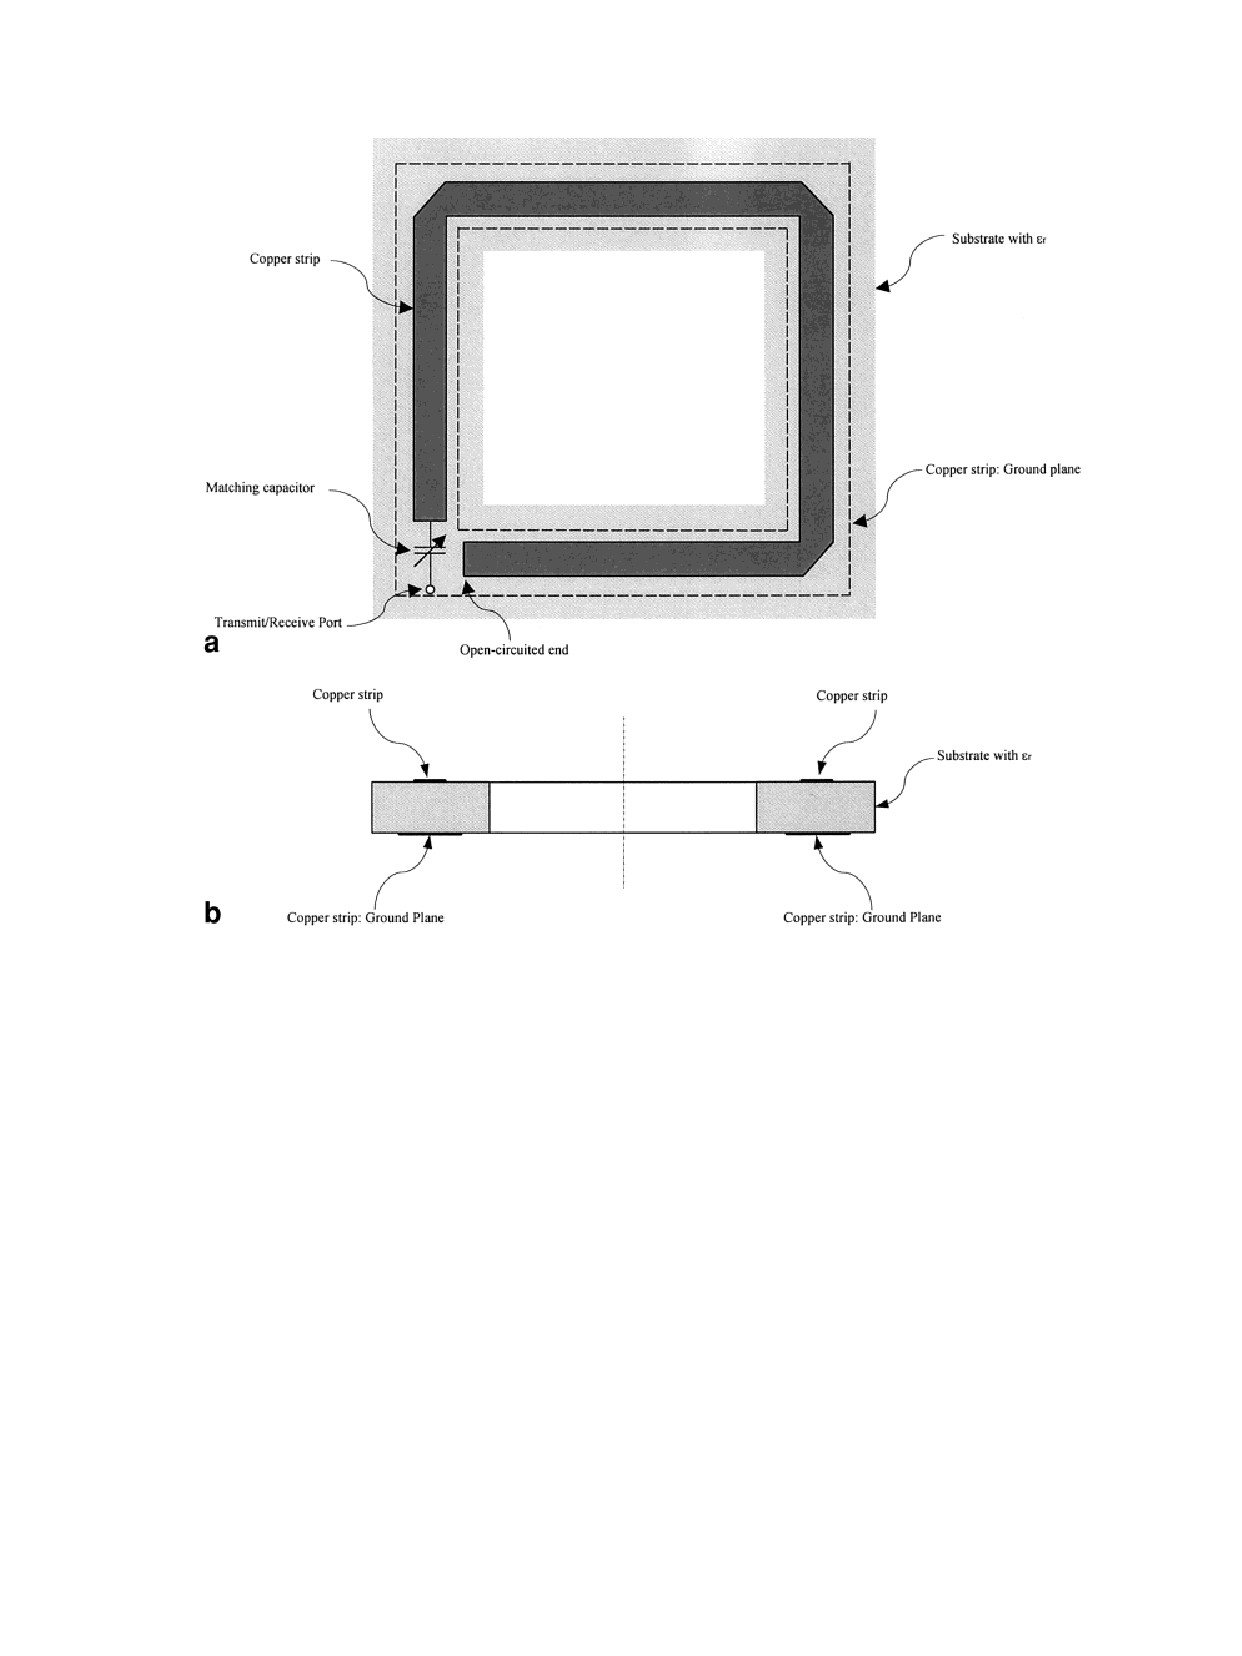
\includegraphics[width=5cm]{Zhang-2001js-F2}
		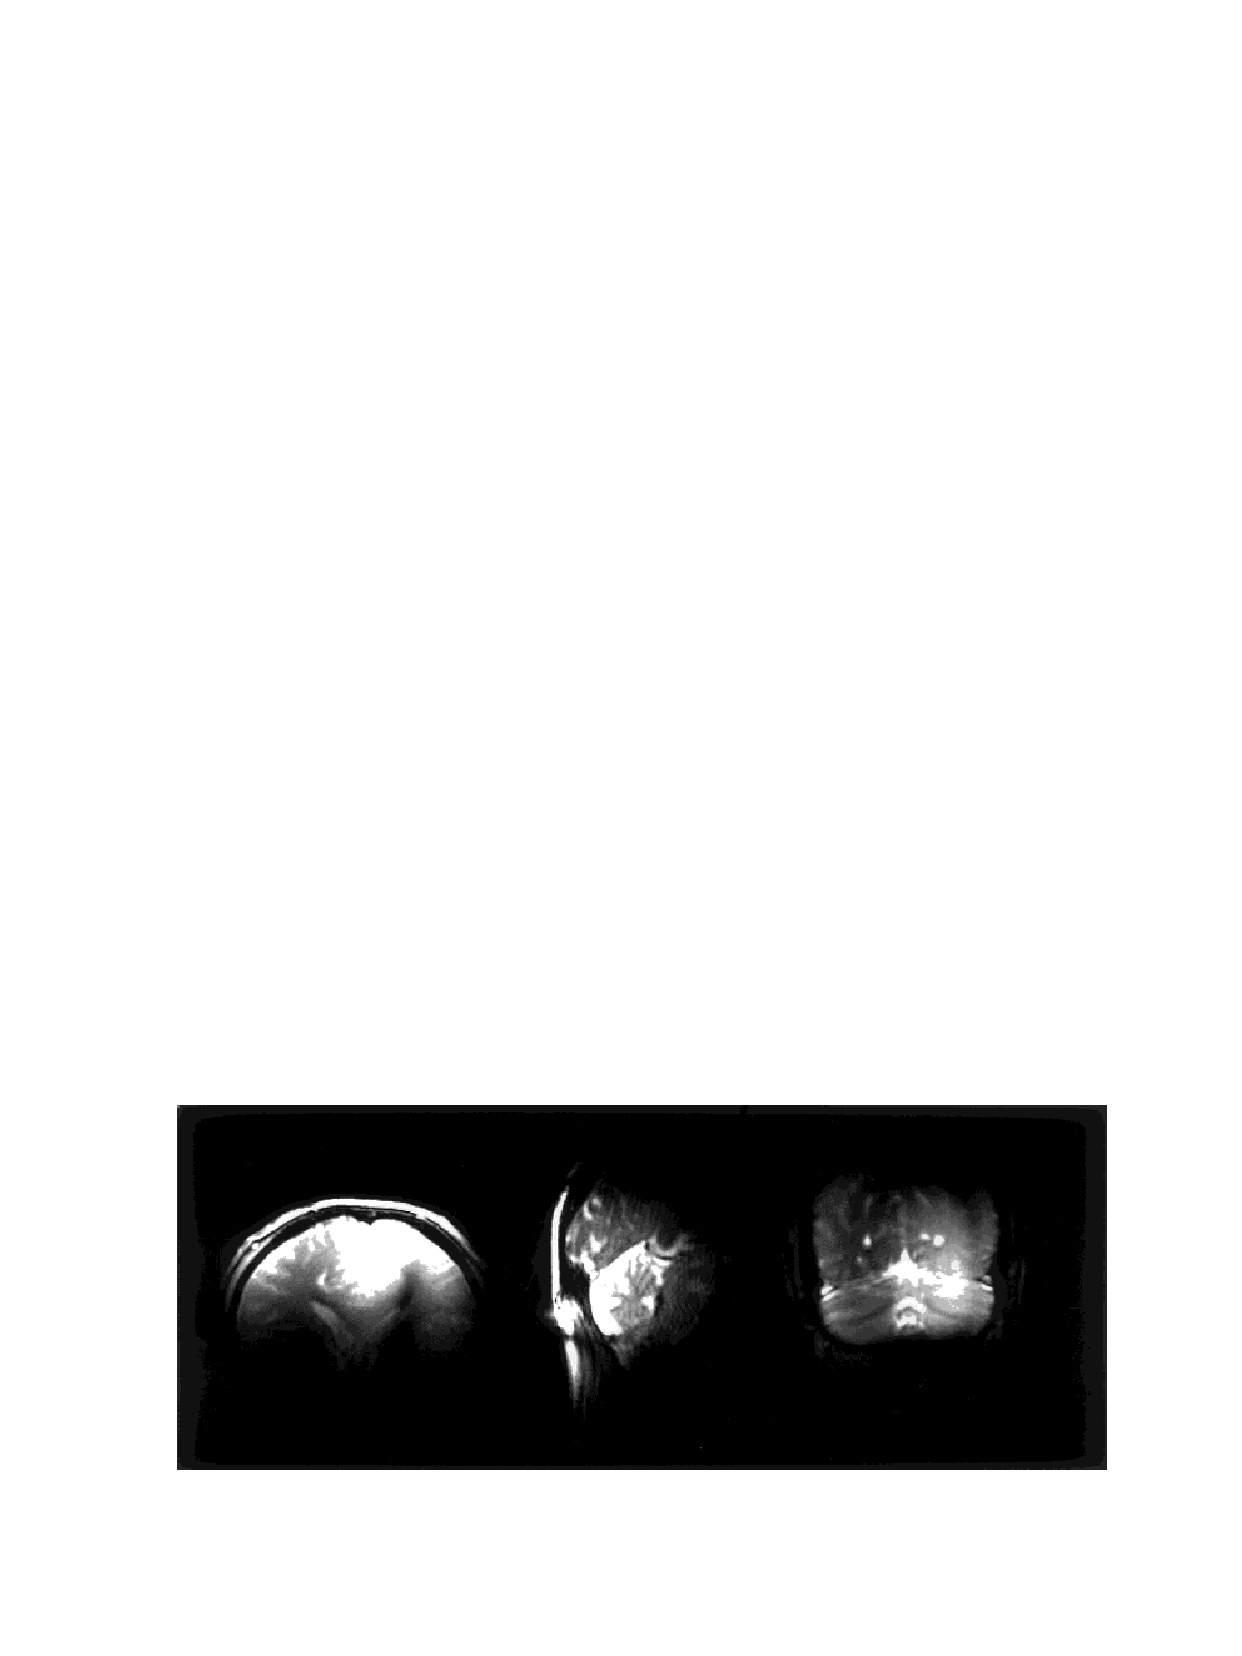
\includegraphics[width=6cm]{Zhang-2001js-F9}
	\end{center}
	\caption{Single-turn microstrip transmission line surface coil for MRI at 7~T (left), and images of the human brain (right). Reprinted with permission from \cite{Zhang:2001js}.}
	\label{fig-Zhang:2001js-F2}
\end{figure}


A similar design has been described later by Bogdanov and Ludwig
\cite{Bogdanov:2002gv}. The arrangement and its eigenmode is similar to the
birdcage coil \cite{Hayes:1985bw}, which has become the mainstay of volume
detectors in MRI. As the magnetic fields available for MRI increased, it
became more important to limit the exposure of the human subject to
radio frequency electric fields. RF heating of the sample, and,
concomitantly induced noise, become more difficult to manage at higher
magnetic fields. With the advent of 3.5~T and later 7~T MRI scanners,
strategies for limiting the penetration of electric fields into the
sample and for reducing radiation losses were needed. Zhang et
al \cite{Zhang:2001js,Zhang:2006wc} demonstrated that single square loop
surface coils made from a microstrip provided significant advantages
over conventional loop coils of comparable dimensions. These loops
consist of a microstrip designed to support a
$\lambda/4$ standing wave, with either
an open or a shorted end. At higher fields, the quarter wavelength
requirement limits the size of the coils that can be built on this
basis. However, planar multi-loop coils supporting higher-order modes
($3\lambda/4$ and higher) have also been
demonstrated \cite{Zhang:2005cr}. 


\begin{figure}
	\begin{center}
		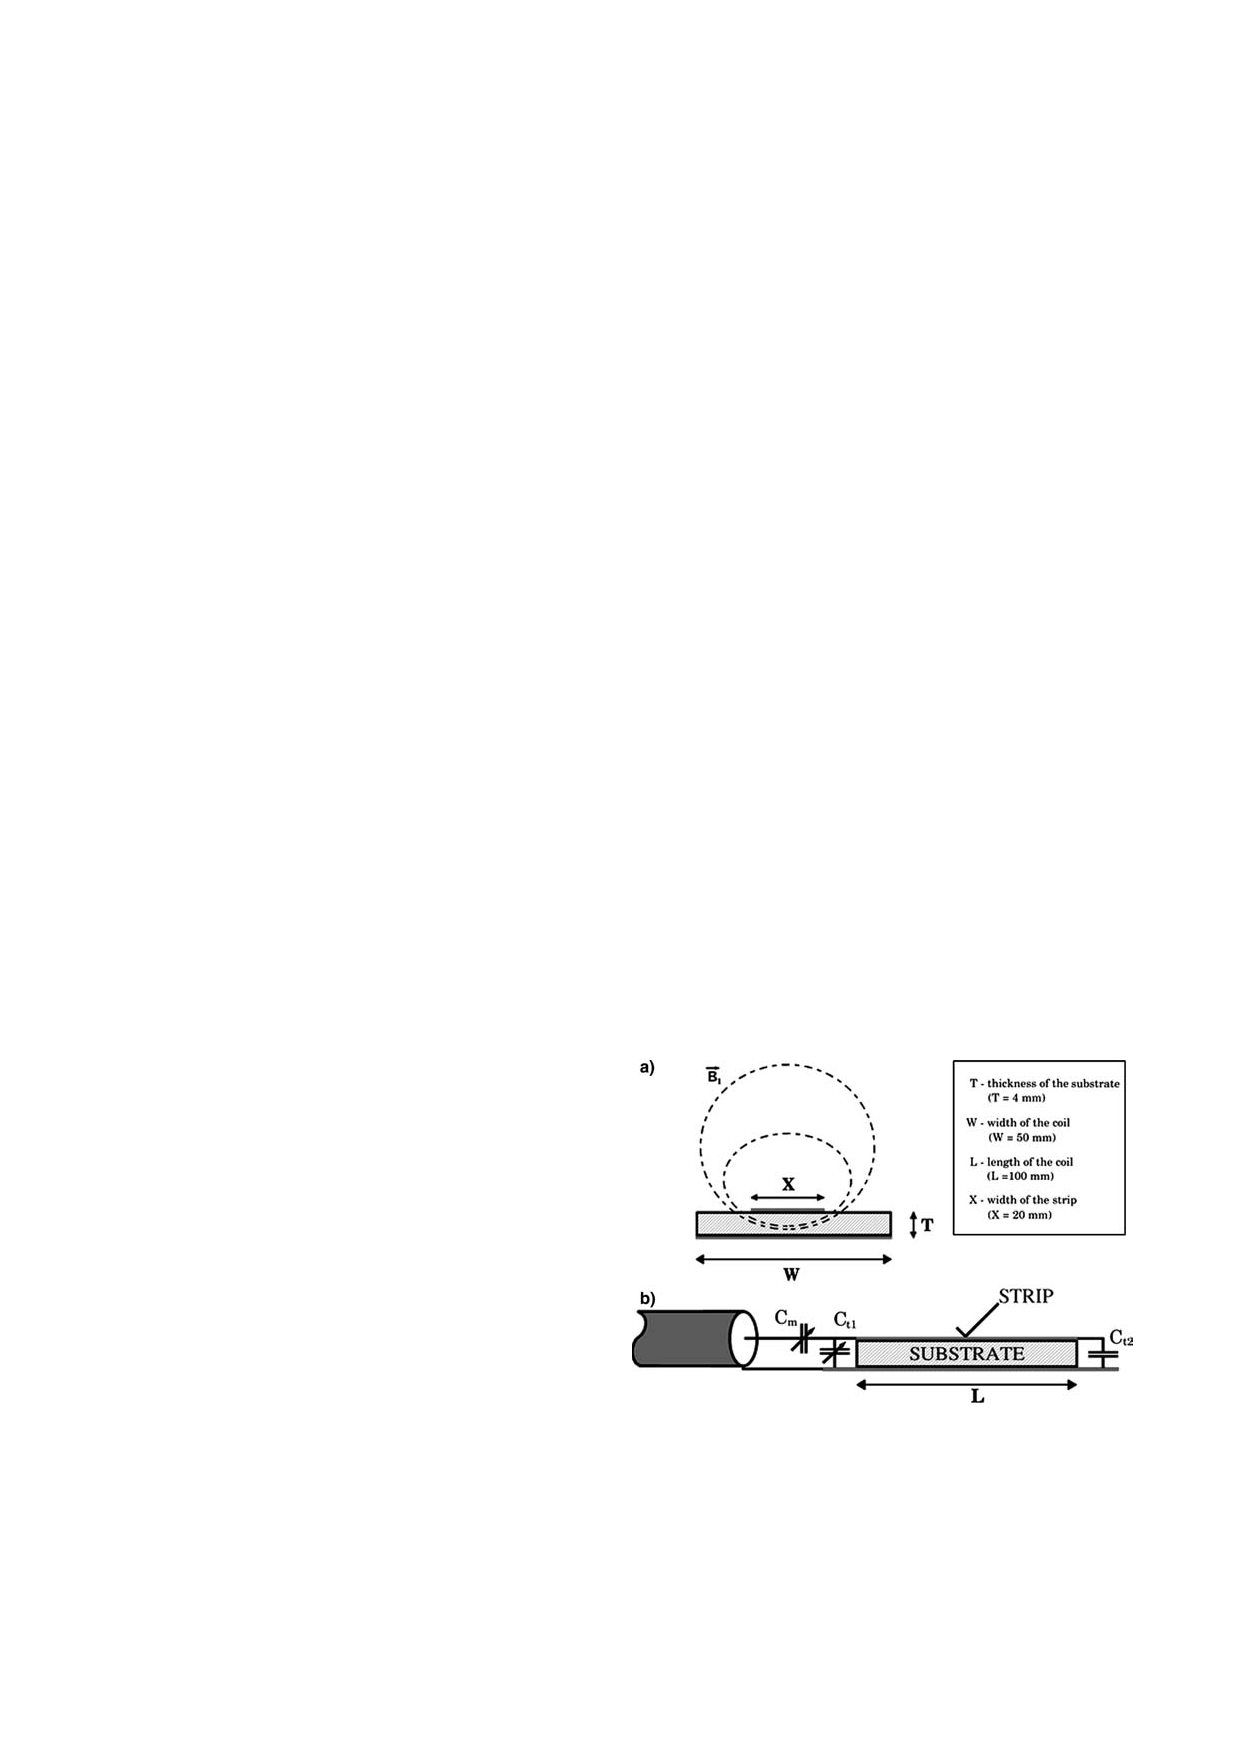
\includegraphics[width=5cm]{Burian-2004fg-F2}
		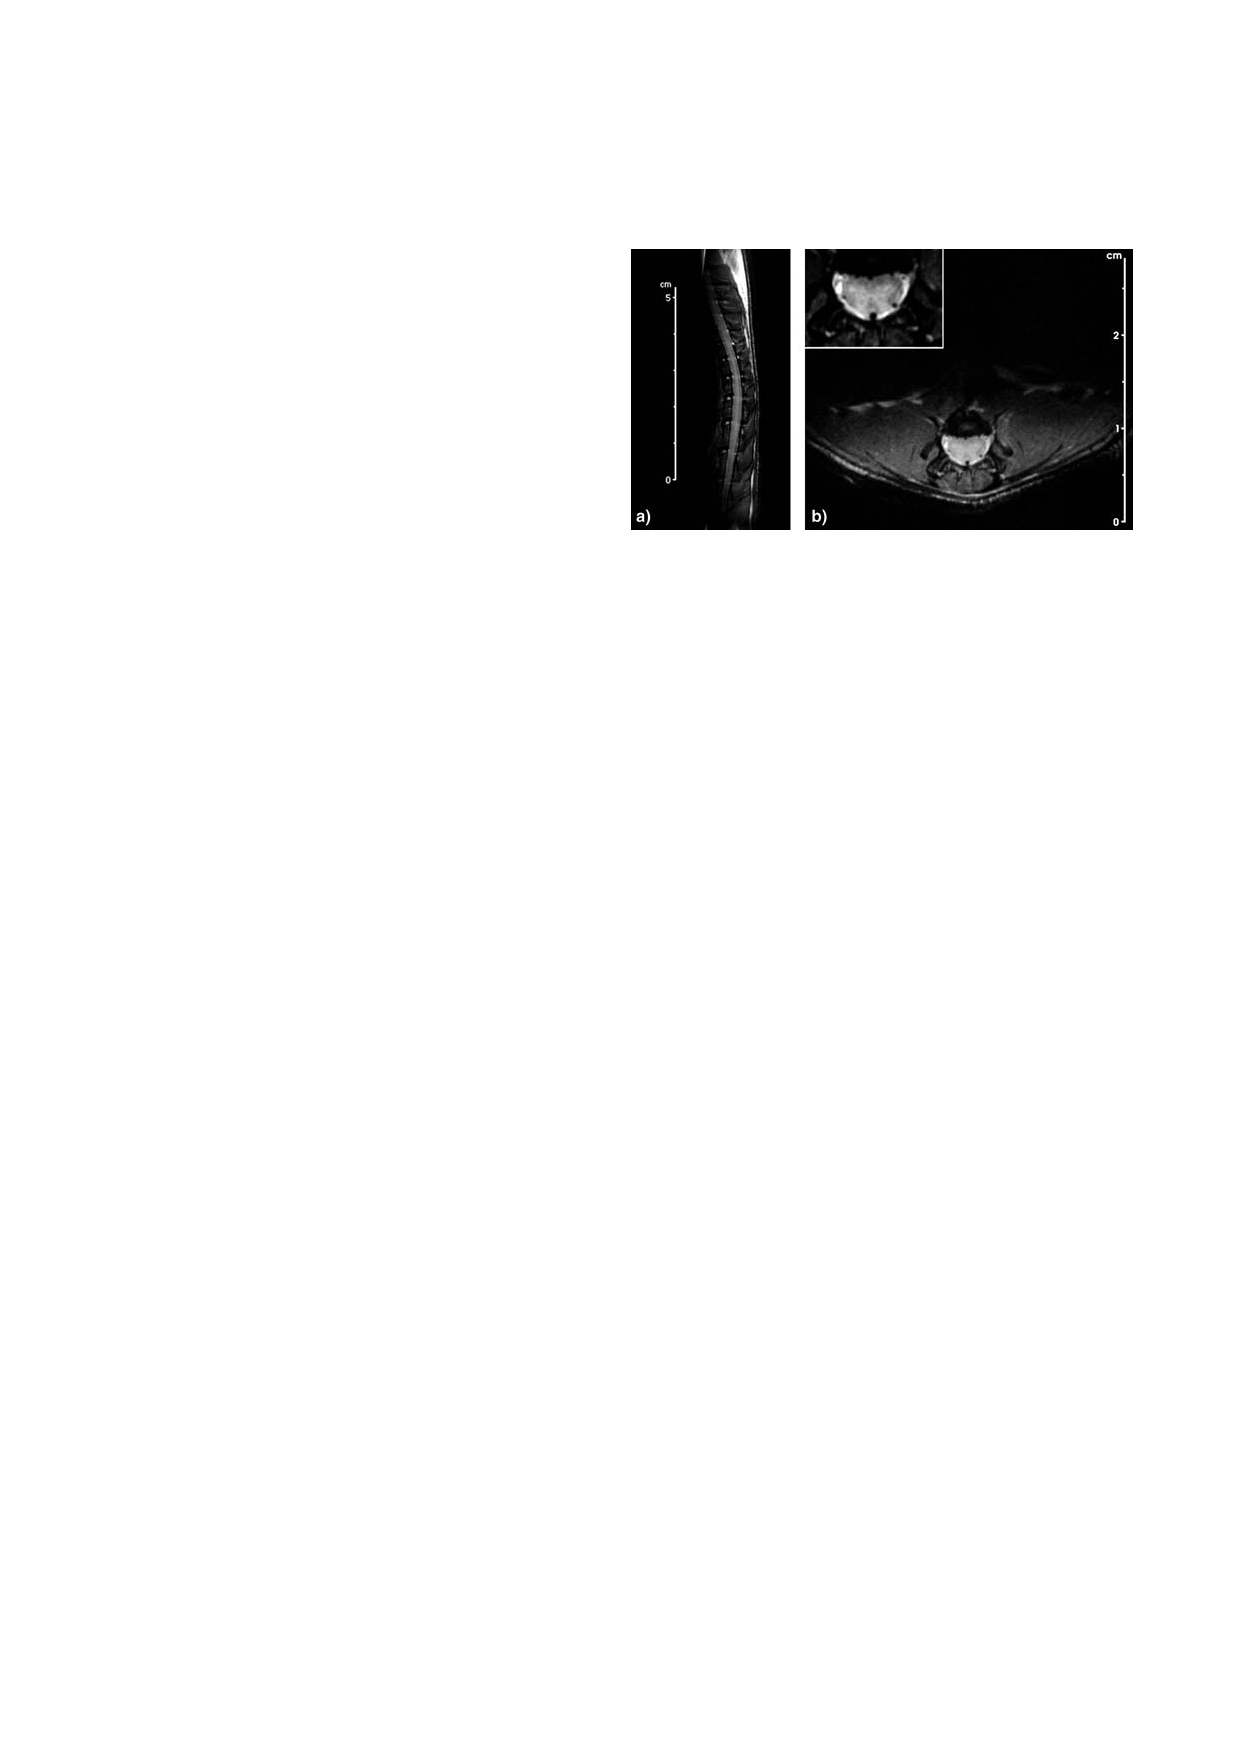
\includegraphics[width=6cm]{Burian-2004fg-F4}
	\end{center}
	\caption{Microstrip transmission line resonator, and images of the rat spine (right). Reprinted with permission from \cite{Burian:2004fg}.}
	\label{fig-Burian-2004fg}
\end{figure}


Zhang et al. developed an elegant version
of the stripline volume detector, in which the coupling between the
lines is accomplished by simply dividing the backplane conductor into
two halves in the axial direction of the cylinder. This avoids the need
to connect each strip separately through a matching network
\cite{Zhang:2003ju}. Standing wave microstrip resonators have been used for
micro-imaging of the rat spinal cord at 4.7~T with a resolution of
0.15mm \cite{Burian:2004fg}, as shown in \fig{fig-Burian-2004fg}. 


Collections of microstrips can be arranged in a three-dimensional fashion
to create volume coils \cite{Driesel:2008di}. 
Actively de-tuneable transmission-line head coils, 
in which the individual microstrips
can be shunted to the ground plane by means of DC-biased PIN diodes
\cite{Vaughan:2002cs}, allow the simultaneous use of localised
receiver coils inside the volume resonator without mutual coupling
artefacts. Lee et al. proposed an array of planar microstrips
\cite{Lee:2001ji,Boskamp:2006tl} for phased-array detection
\cite{Roemer:1990gs,Hoult:2004gm}. Their design exploits an intriguing
property of identical parallel and coplanar microstrips: standing wave
modes in adjacent strips are automatically decoupled from each other by
symmetry. Phased microstrip array detectors have since been used
successfully as external coils for prostate imaging
\cite{vandenBergen:2010hg}, and an array of mutually decoupled microstrip
loops has been used by Adriany et al for parallel acquisition and
individual control of RF phases and amplitudes in a human head coil at
7~T \cite{Adriany:2005cw}. It should be noted that in cylindrical and other
non-planar arrangements, identical parallel microstrips are no longer
automatically decoupled. Decoupling can be achieved either capacitively,
or inductively \cite{Wu:2006bs}; the latter approach has the advantage that
the coupling and decoupling mechanisms follow the same frequency
dependence, i.e., the decoupling is broad-band. 

The properties of
microstrip resonators and other MRI detector geometries have been
compared in numerical and in some cases experimental studies by several
authors \cite{Wang:2006gk,vandenBergen:2009dk,Ipek:2012bm}. Wang and Shen
\cite{Wang:2006gk} compared the sensitivity, power deposition, and field
distributions for birdcage, microstrip, and TEM coils at 7T by finite
element computations. They found microstrip coils to provide superior
SNR while depositing less power into the tissue than birdcage or TEM
resonators. Ipek et al. \cite{Ipek:2012bm} experimentally compared a
radiative dipole antenna with a microstrip resonator of similar
dimensions for prostate imaging at 7T. The radiative antenna design is
optimised to produce a Poynting vector perpendicular to the plane of the
antenna, in order to radiate into the tissue and reach deeper lying
structures. By contrast, the microstrip resonator does not radiate
efficiently, the main direction of its Poynting vector is in the axial
direction (and its time average vanishes due to the standing wave
resonance). Ipek et al. found this to be reflected in deeper reaching B1
fields for the antenna. However, the power deposited in the tissue was
lower, and the SNR for areas closer to the receiver was higher for the
microstrip resonator. 

\subsection{Microfluidic NMR}
Micro-solenoid coils, with diameters more than an order
of magnitude smaller than conventional detectors, exhibit very high mass
sensitivity \cite{Olson:1995vu,Sweedler:1997tl,Lacey:1999vk}, and thus allow
direct combination of NMR detection with
chromatographic separation techniques such as
capillary electrophoresis \cite{Peck:1994hh,Wu:1994ks,Olson:1999ed} and
high-pressure liquid chromatography \cite{Lacey:2001dr}. Solenoidal micro
coils have also been used successfully for micro-imaging
\cite{Seeber:2000iy,Ciobanu:2002wo}, achieving resolutions approaching the
single cell length scale. 

In solid-state NMR, micro coils have been used
for statically, for example for studying spider silk
\cite{KYamauchi:2005jv}, but also under Magic-angle spinning (MAS) NMR has
been made possible by attaching the micro-scale sample to a conventional
MAS rotor, and surrounding it by a micro-solenoid \cite{Kentgens:2008ch}.
Another possibility is to insert a tuned micro coil into the MAS rotor,
and spinning it together with the sample. The coil is then inductively
coupled to the macroscopic probe coil
\cite{sakellariou2007hrh,Jacquinot:2011cj}. 

In recent years, MAS probes
capable of very high spinning speeds, exceeding 100kHz, have been
demonstrated, and are now commercially available. In these systems, the
sample diameter has to be kept small in order to limit the inertial
forces. This has inevitably led to smaller and smaller samples, and the
dimensions of the rotors and coils of the most recent designs approach
those of the micro-solenoids that were introduced for liquid-state NMR
in the 1990s \cite{Samoson:2010et}. 

Solenoid micro coils have also been
used for remote detection in the context of microfluidic devices. In
this elegant approach, position, velocity, and in some cases, chemical
information is encoded into the spin phase and polarisation inside
microfluidic system, by way of a macroscopic coil which surrounds it.
The fluid then flows out of the microfluidic device, and is led in a
capillary through a micro coil, where the NMR signal is recorded. In
this way, the velocity distribution as well as chemical reaction
dynamics in microfluidic systems have been characterised in real time
\cite{Hilty:2005eq, McDonnell:2005dn,Harel:2007bs, Bouchard:2008hv,
Ledbetter:2008kp,Harel:2009eg,Bajaj:2010cy,Telkki:2011wi,Telkki:2014jf}.

\subsection{Planar Detectors}\label{nmr-and-microfluidics-planar-detectors}
With the success of miniaturised solenoid coils, it became conceivable
to integrate NMR spectroscopy with emerging microfluidic lab-on-a chip
technology. Typical sample volumes in microfluidics, ranging from a few
$\mu$l down into the pl range, are comparable to the volumes of some of
the micro-solenoids that had proven superior mass sensitivity
performance in hyphenated chromatography-NMR integrations. However,
Lab-on-a-chip devices are typically planar, fabricated through
lithographic processes, and the liquid volumes they contain are
separated from each other by relatively large distances. Integrating
solenoid coils into such structures, while not impossible, presents
significant fabrication challenges \cite{Badilita:2010hb}. As a possible
solution, planar spiral coils were explored extensively. The first
demonstration, by Stocker et al. \cite{Stocker:1997by}, placed a sample
droplet directly in contact with the micro coil. Trumbull et al.
integrated a single loop inductor with a microchip-electrophoresis
system \cite{Trumbull:2000fa}. The loop inductor
was fabricated through a lift-off process, and the metal thickness 
was therefore less than 1 $\mu$m. Since this is below the skin depth, it
probably limited the sensitivity of the system. It was found that
microfluidic chips made from polyimide provided
considerably better spectral resolution than those made from pyrex glass,
 probably due to the closer
 match in susceptibility between the polyimide and water. While NMR
spectra of test samples were successfully collected, the sensitivity of
the device was not found to be sufficient for a credible integration
with capillary electrophoresis. 

Later implementations involved
fabrication of the spiral coil structure by lift-off lithography and
subsequent electroplating onto a glass microfluidic chip
\cite{Massin:2002bj}. This allows thicker conductors, significantly
reducing ohmic losses. Microfluidic probes based on this design
\cite{massin2003pmb} reached limits of detection of 260~$\mathrm{nMol\,\sqrt{s}}$ 
at 470~nL probe volume, and 20~$\mathrm{nMol\,\sqrt{s}}$ at 30~nL (values
scaled to 600 MHz proton frequency). However, the spectral resolution
was quite poor, insufficient to resolve homonuclear $J$ couplings in the
\chemical{^1H} spectra. This was probably due to the circular shape
of the sample chamber that was used.

 Better resolution was achieved
by arranging it in a linear channel aligned with the magnetic field
\cite{Wensink:2004kd}, making it possible to monitor the on-chip
condensation of benzaldehyde and aniline \cite{wensink2005mrk}; further
applications of planar spiral coil designs to microfluidic reaction
monitoring followed \cite{Gomez:2010jr,Yue:2012fw}. Planar spiral coils
have also been applied to EPR spectroscopy \cite{Boero:2003hf} at the micro
scale.

Placing planar coils on both sides of the sample leads to the
concept of micro-Helmholtz coils. These provide potentially high
sensitivity and B1 homogeneity, but present considerable fabrication
challenges. An elegant implementation has recently been described by
Spengler et al. \cite{Spengler:2014ir,Spengler:2016km}. Phased arrays
provide another potential approach to planar micro-NMR detectors. A
proof of concept has been given by Gruschke et al, who have demonstrated
a system of 7 partially overlapping coils fabricated using a
wire-bonding process \cite{Gruschke:2012df}. This detector has been used
successfully to image human skin samples \cite{Gobel:2014tf} and to study
porous media using a single-sided, permanent magnet spectrometer
\cite{Oligschlager:2015fl}.

\begin{figure}
	\begin{center}
		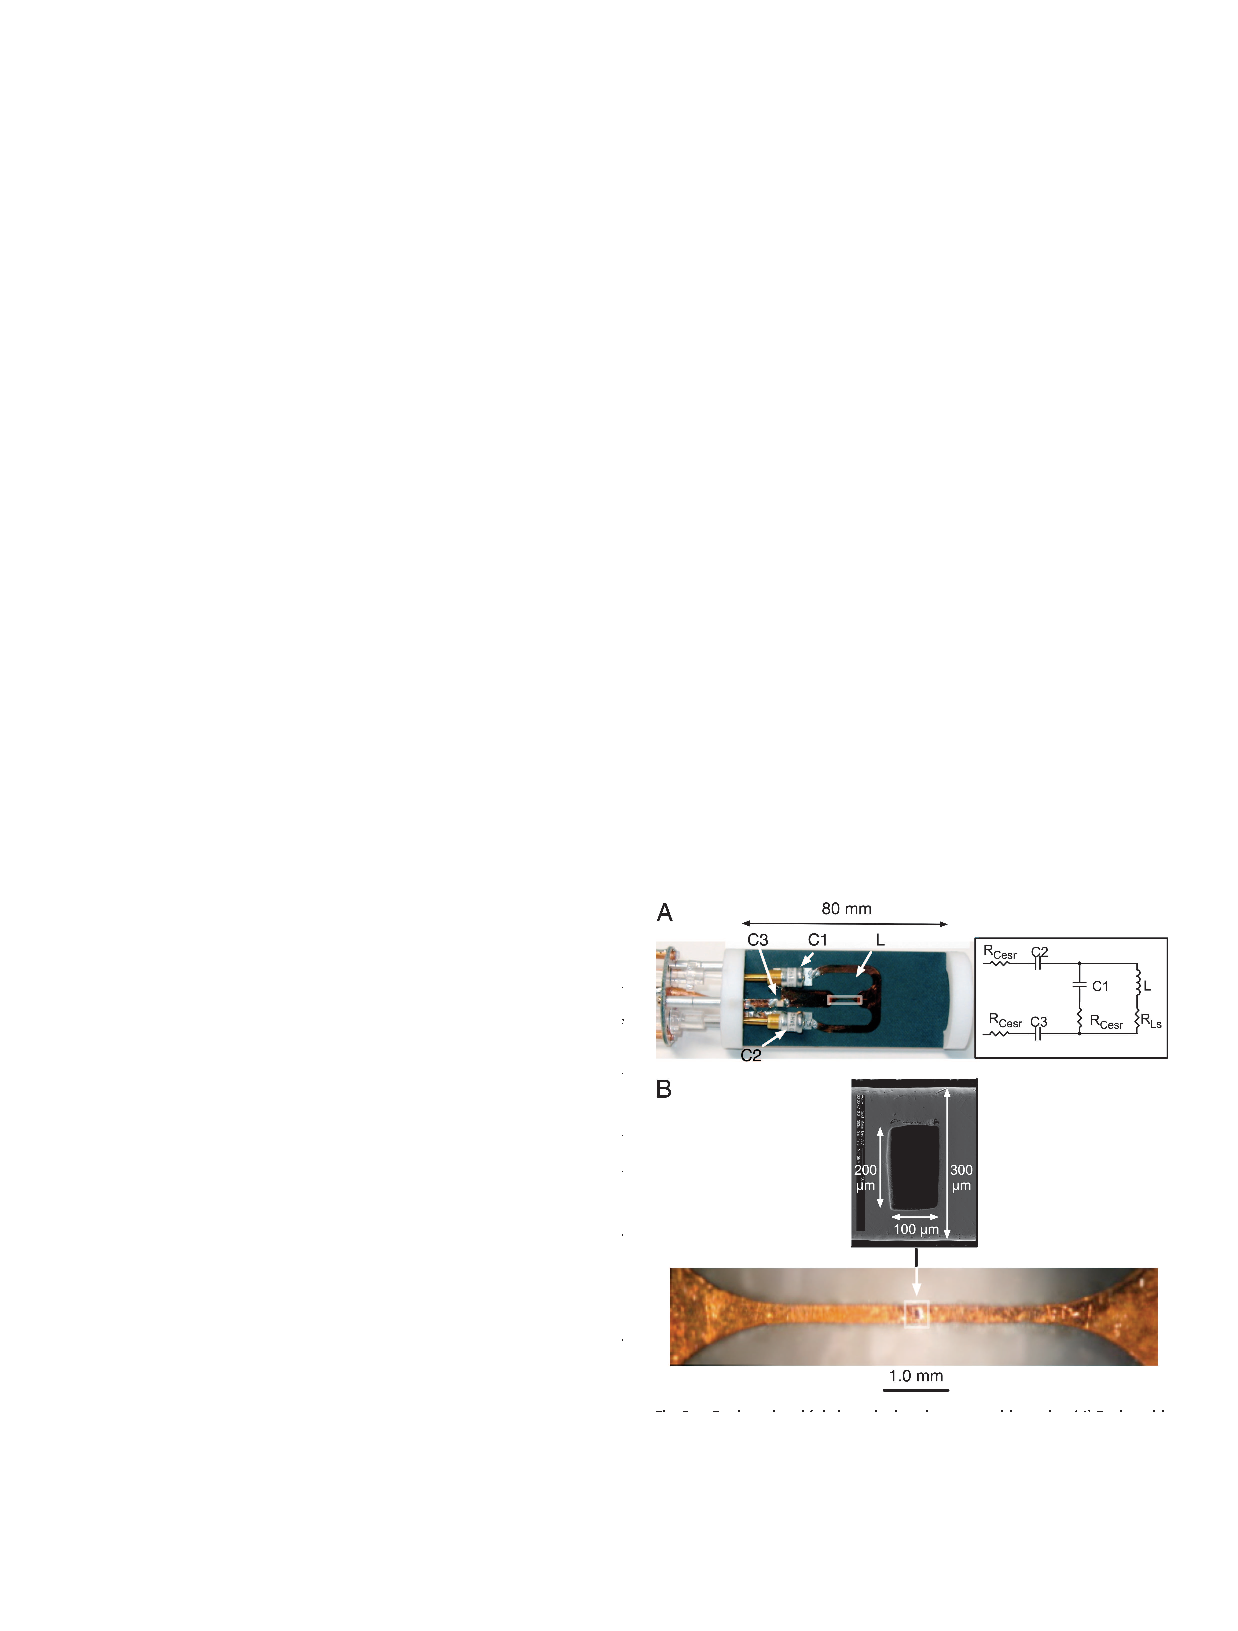
\includegraphics[width=5cm]{Maguire-2007ko-F2}
		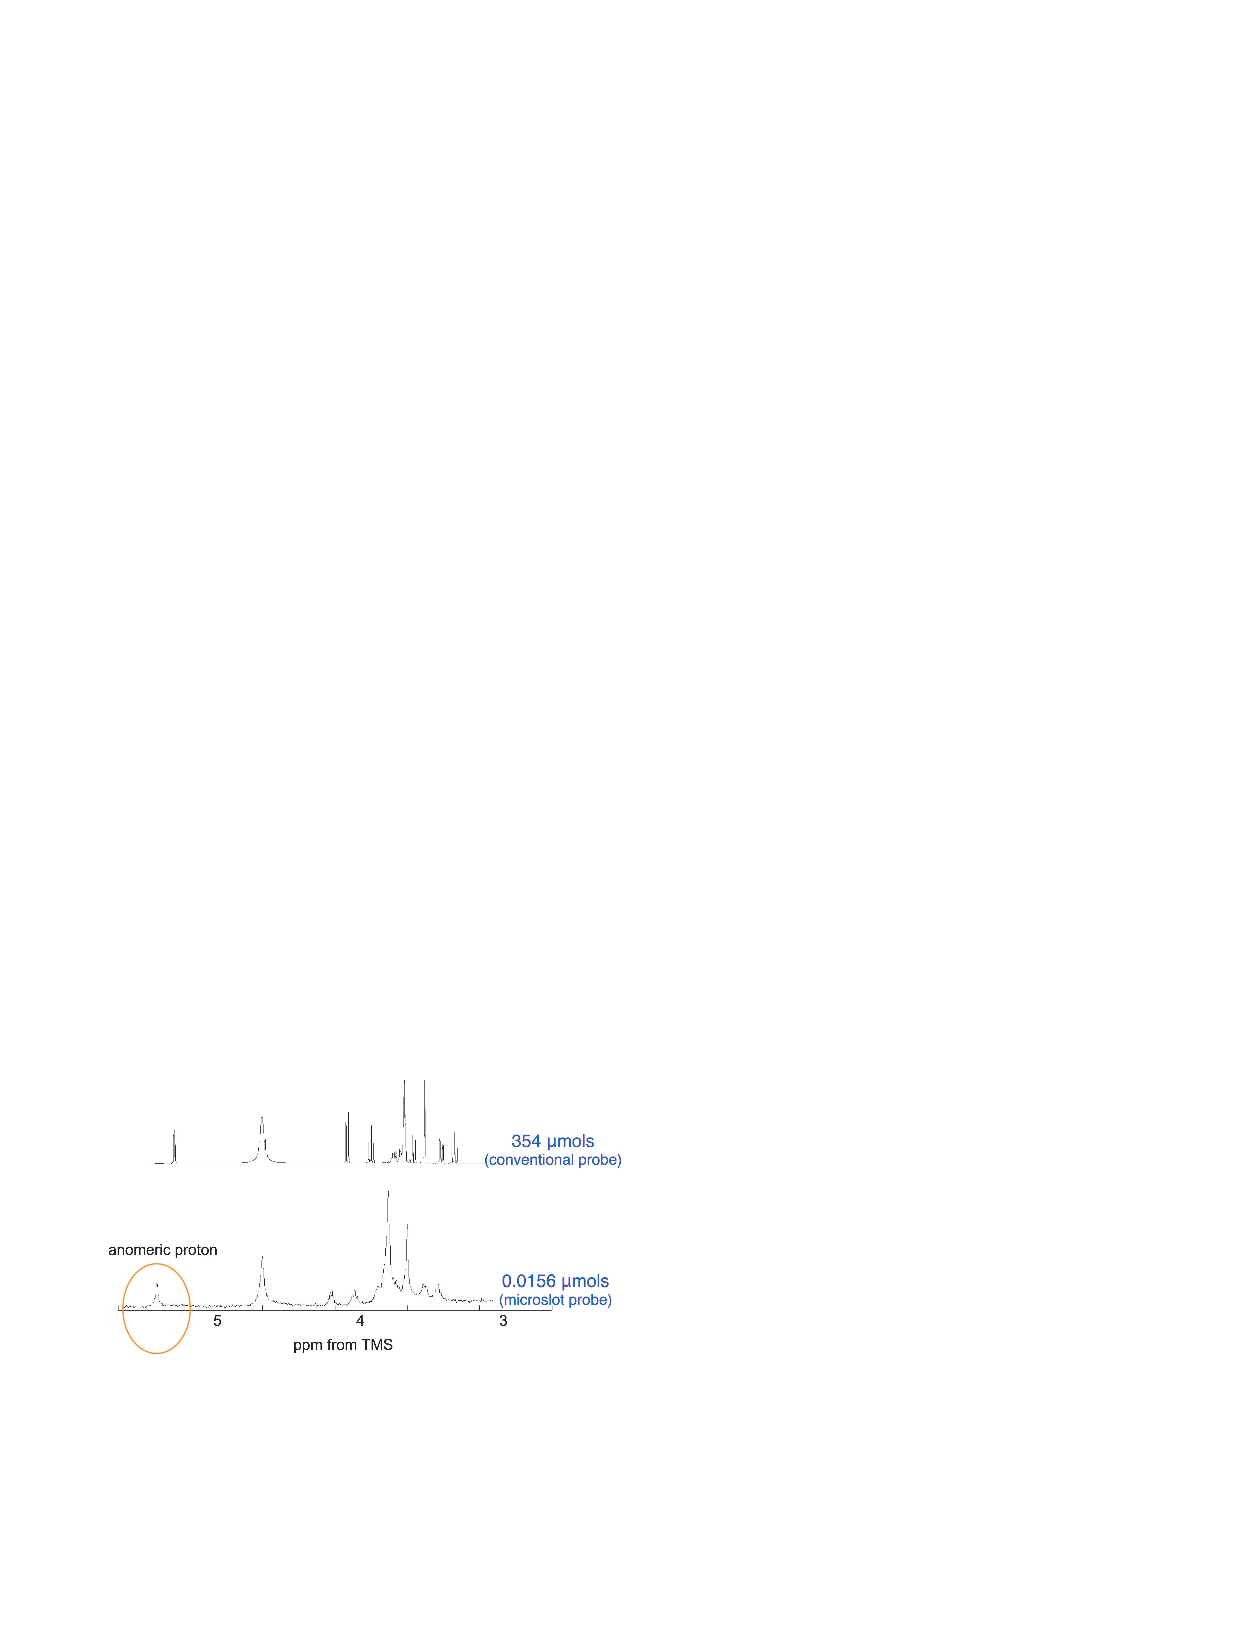
\includegraphics[width=6cm]{Maguire-2007ko-F4}
	\end{center}
	\caption{Left: Microslot probe. A: Probe with housing removed, B: Scanning electron micrograph and light micrograph of the slotted microstrip detector. Right: Spectrum of sucrose in \chemical{H_2O} acquired with a conventional (top) and the slotted microstrip probe (bottom).  Reprinted with permission from \cite{Maguire:2007ko}.}
	\label{fig-Maguire-2007ko}
\end{figure}


\subsection{Microstrip Detectors}
Given the difficulty of integrating three-dimensional coils with planar
microfluidic devices, and the benefits that linear structures aligned
with the B0 magnetic field offer in terms of field homogeneity, it is
not surprising that microstrip detectors were considered for integrating
microfluidics and NMR. A problem that arises immediately is that
transmission line resonators require longitudinal dimensions that are of
the order of the wavelength, which amounts to tens of centimetres for
typical NMR Larmor frequencies. Maguire et al. therefore proposed
slotted microstrips as a means to concentrate the RF magnetic field, and
therefore the sensitivity, to a mm-sized area
\cite{Maguire:2009wc,Maguire:2007ko}. Their design was based on a single
microstrip conductor of 0.3 mm width and about 5 mm length, fabricated
using RF printed circuit board material using standard wet-etching
techniques (\fig{fig-Maguire-2007ko}).

At the centre of this structure, a square-shaped piece of
the Cu conductor was removed from the microstrip. This concentrates the
current into the narrow remaining conductor bridges, and leade to a
corresponding increase in local magnetic field. As a result, the mass
sensitivity is significantly better than what had previously been achieved
with spiral planar coils. 

\begin{figure}
	\begin{center}
		\begin{tikzpicture}
			\node at (-2,0) {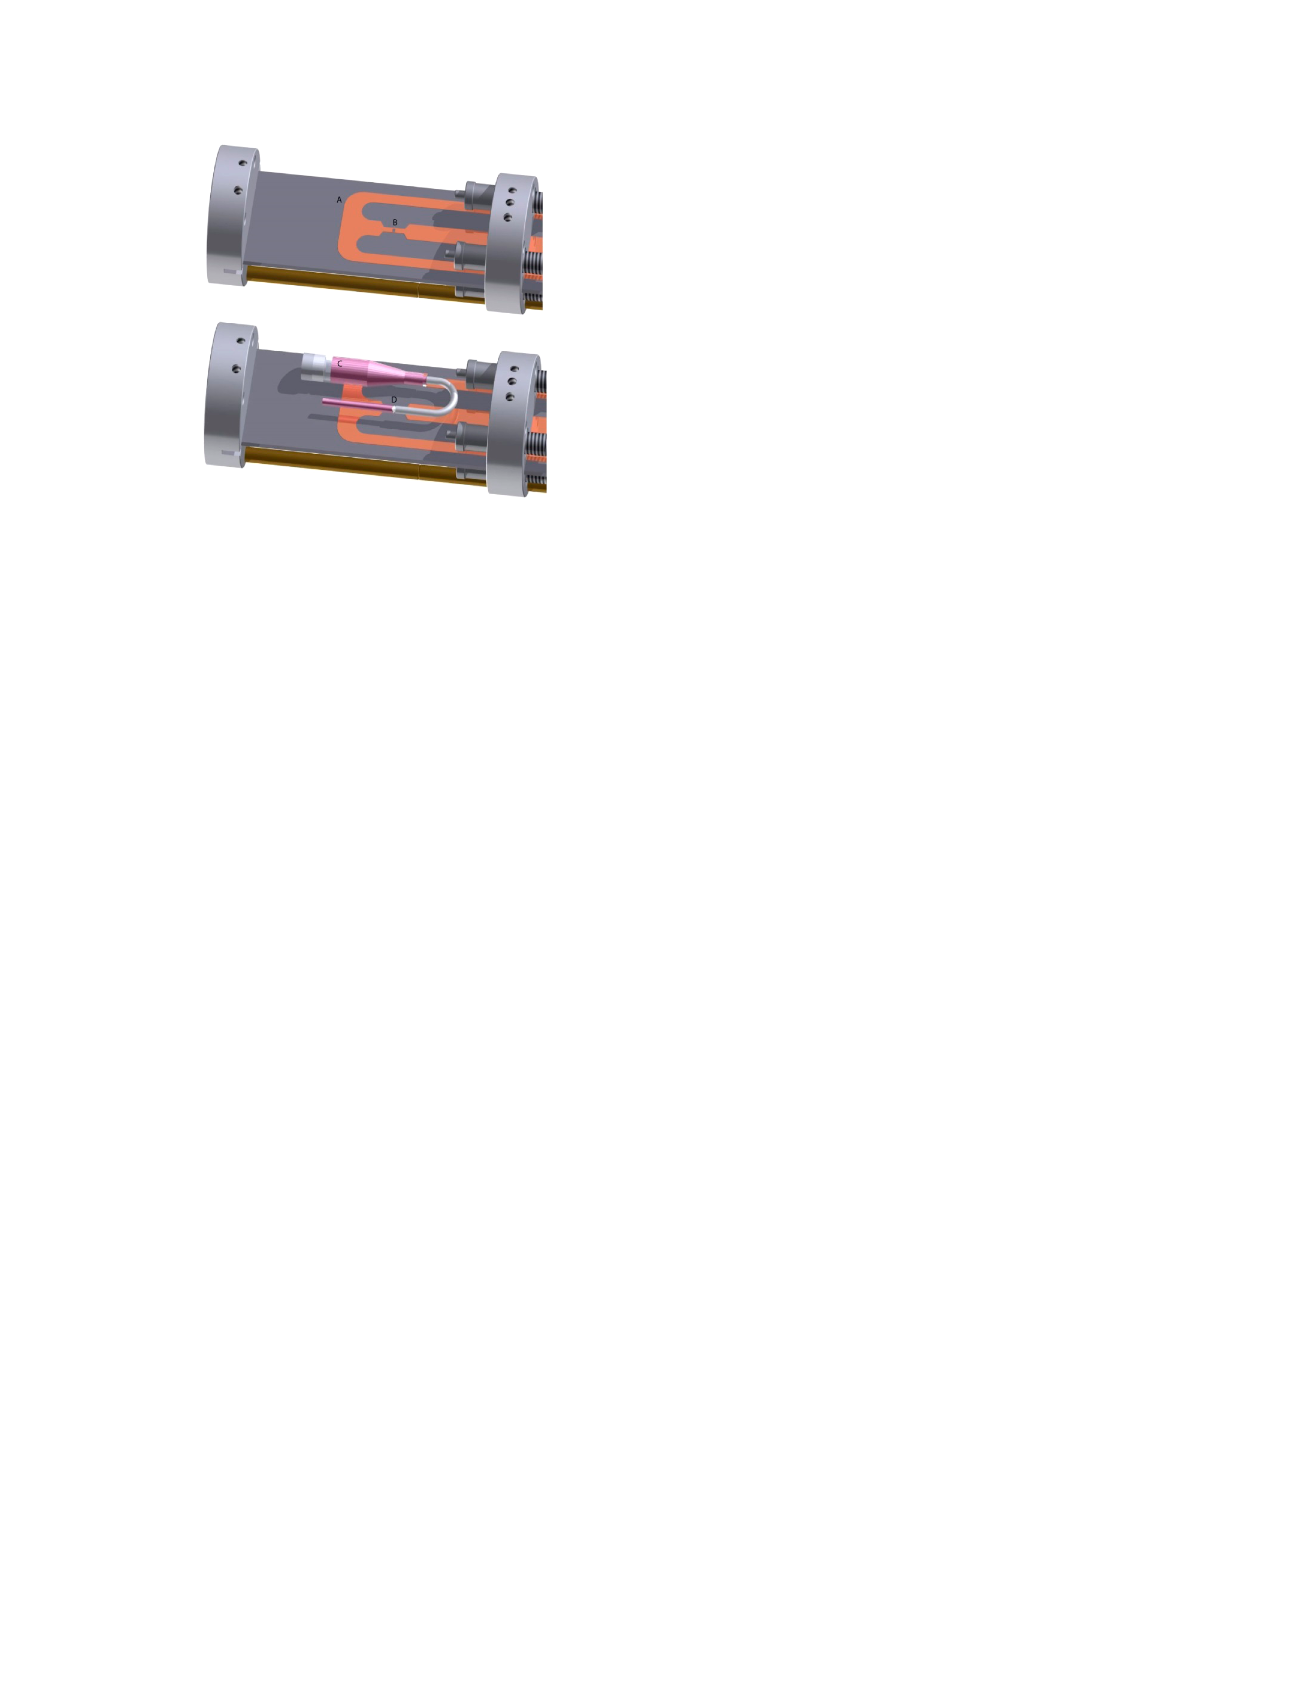
\includegraphics[height=3cm]{Kalfe-2015ik-F3}} ;
			\node at (-3.5,1.5) {A} ;
			\node at (2,0) {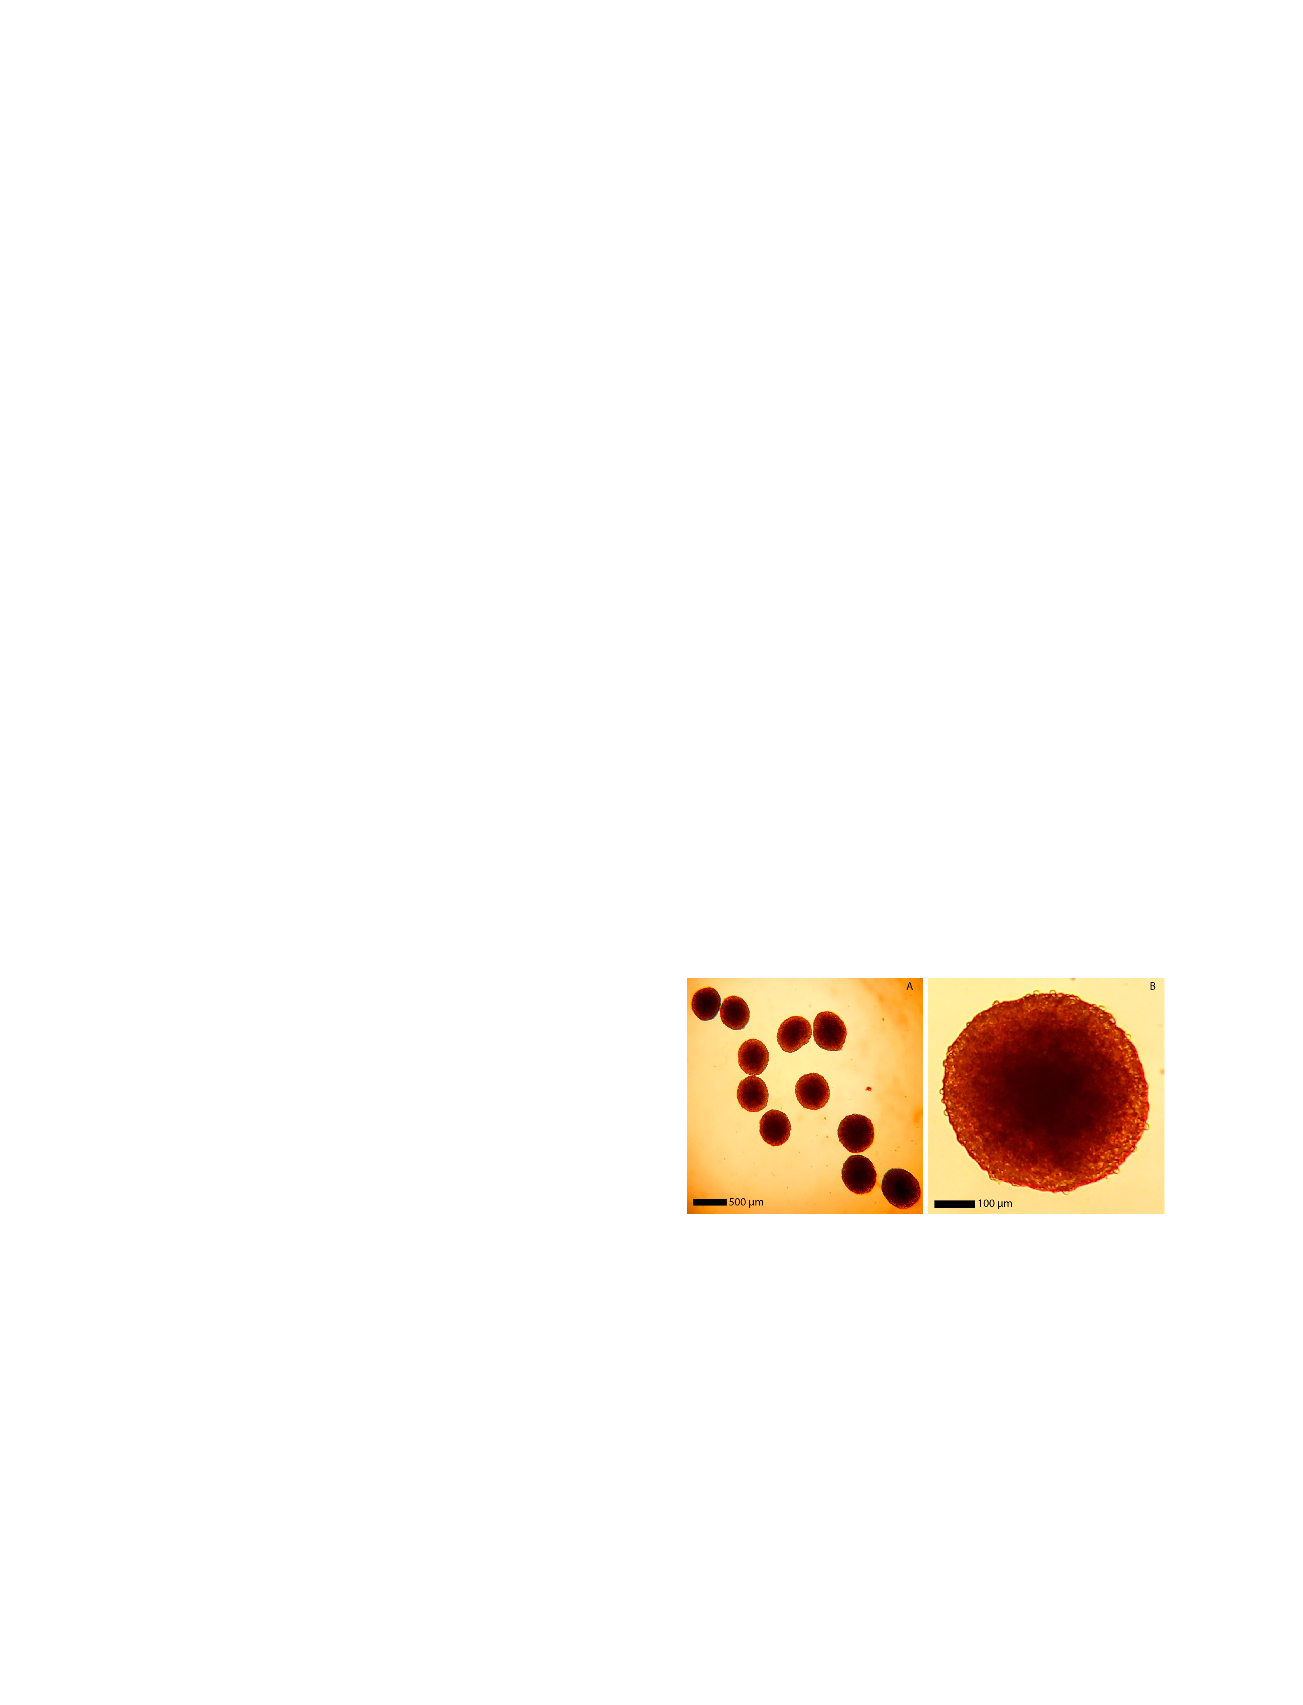
\includegraphics[width=3cm]{Kalfe-2015ik-F1}} ;
			\node at (0.5,1) {B} ;
			\node at (0,-3) {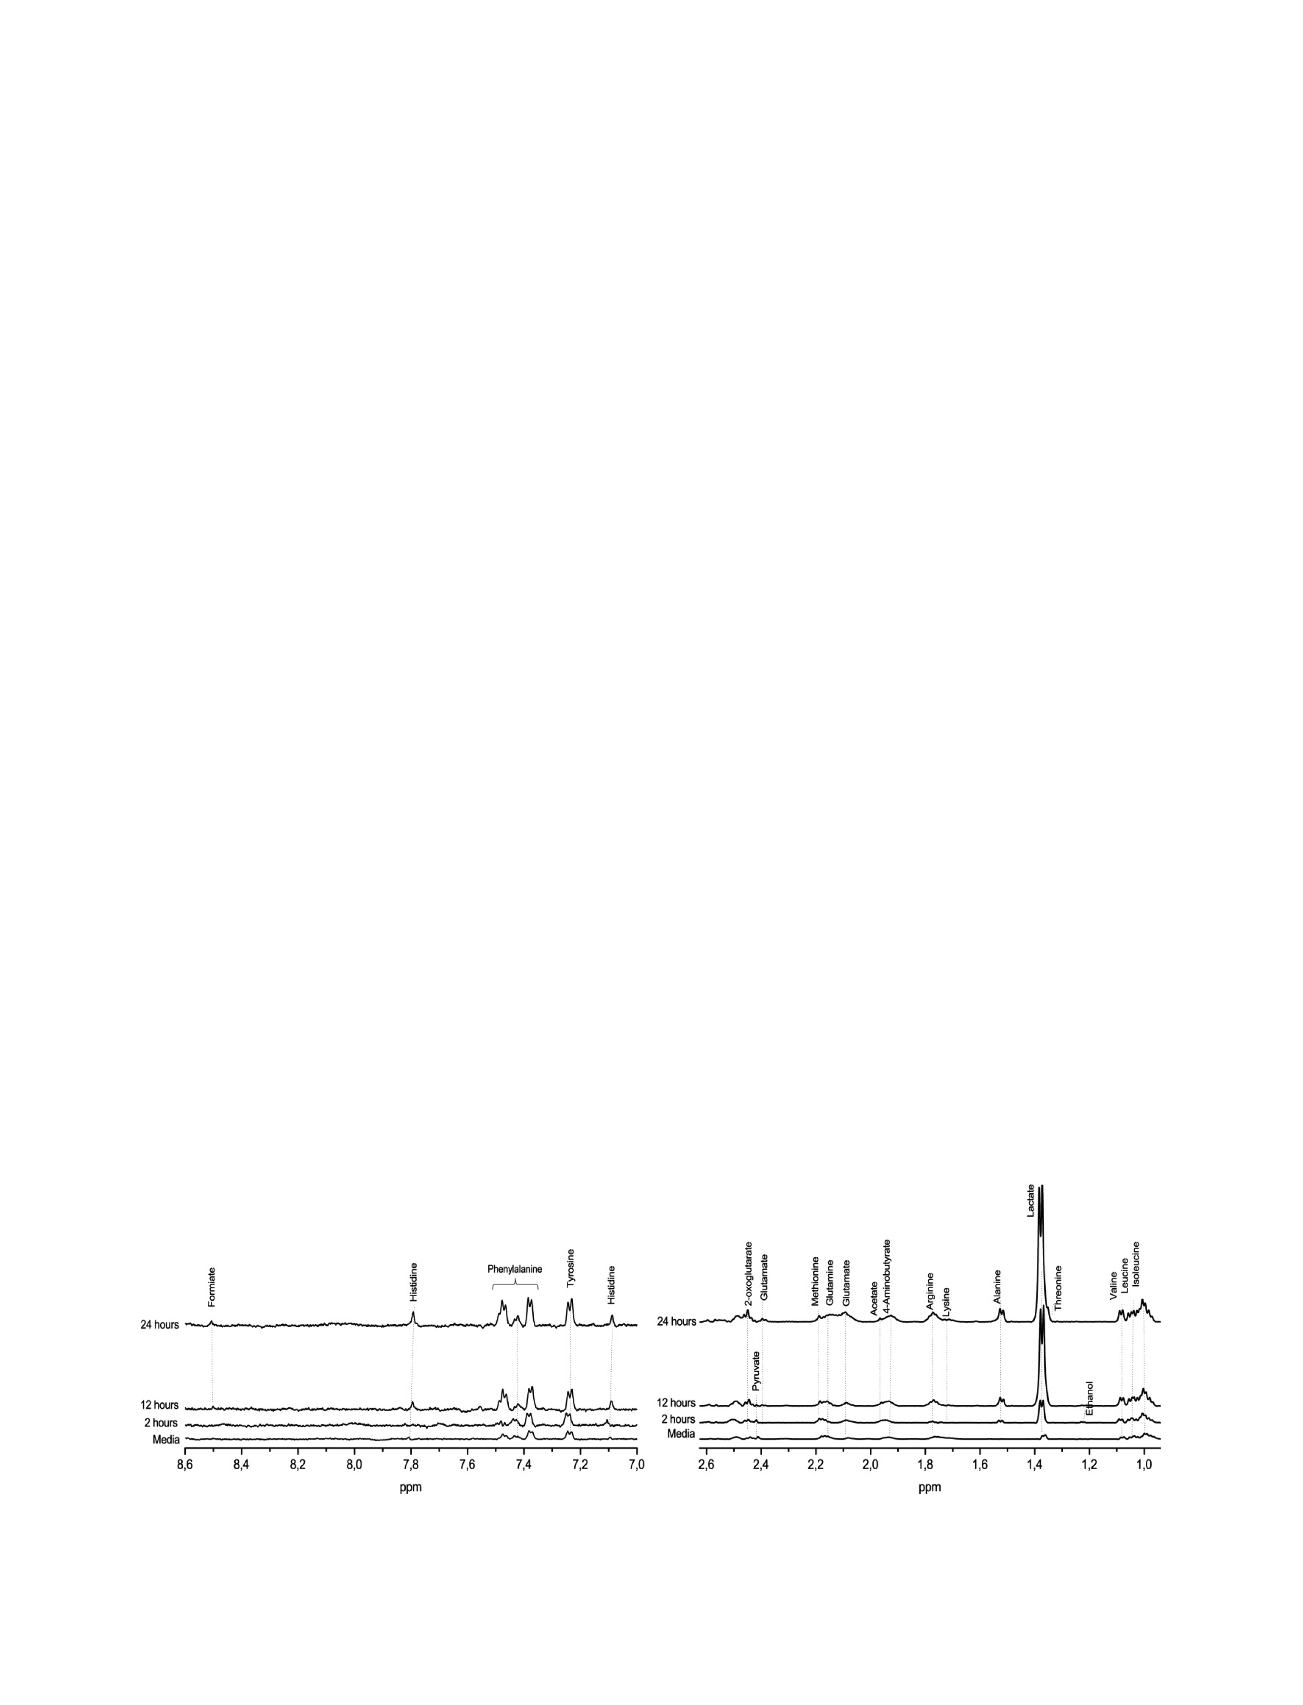
\includegraphics[width=10cm]{Kalfe-2015ik-F4}} ;
			\node at (-4.5,-2) {C} ;
		\end{tikzpicture}
	\end{center}
	\caption{Tumour spheroid microdevice. A: CAD rendering of the microslot probe without (top) and with
	(bottom) the culture device in place; B: Optical micrographs of tumour spheroids; C: 600 MHz \chemical{^1H} NMR
	spectra obtained with the system. Adapted with permission from \cite{Kalfe:2015ik}.}
	\label{fig-Kalfe-2015ik}
\end{figure}

		At the same time, a half-height line width of
about 1.1~Hz was obtained, significantly superior to any other planar
micro-NMR detector described up to that point. However, the baseline
resolution was still relatively poor (\textgreater{}50 Hz at 0.5\%).
Nonetheless, one- and two dimensional 1H NMR spectra of sucrose and of
ribonuclease A were obtained successfully. Microslot probes of this type
have since been applied successfully for studying the metabolism of
biological systems. In one of the first credible demonstrations of
microfluidic NMR metabolomics, a microslot detector was applied to
obtain NMR spectra of a metabolite concentrate from a cell line by
Krojansi et al \cite{krojanski2008mnp}. More recently, the exa-metabolome
of a tumour spheroid was observed directly by combining the microslot
detector with an evaporation-driven perfusion micro-device
\cite{Kalfe:2015ik}, as shown in \fig{fig-Kalfe-2015ik}.

\subsection{Non-Resonant Detectors}
The microstrip geometry
has also been used to build non-resonant NMR saddle coils
\cite{Murphree:2007hg}. In this approach, a saddle coil is defined by
microstrips fabricated on a flexible printed circuit board, which is
then wrapped in a cylinder to serve as a saddle-coil NMR probe. The
microstrips are designed to have a specific impedance of 50$\Omega$, and are
terminated by a 50$\Omega$ resistor between the microstrip and ground
conductors. Unlike typical NMR detectors, this system does not rely on
an electromagnetic resonance (standing wave) in order to couple the
detector to the transmitter/receiver system \cite{Mispelter:2006ty}. Instead,
a travelling TEM wave is directly coupled to the precessing nuclear
spins. The most notable advantage of this approach, commonly referred to
as travelling-wave NMR, is its broad-band nature, which makes it simple
to perform multinuclear NMR experiments. The saddle coil system
mentioned above has been used, without re-tuning, to obtain \chemical{^1H}, 
\chemical{^{13}C},
\chemical{^{19}F}, and \chemical{^{31}P} spectra at 0.52~T. 
Broadband switching between transmission
and receiver mode has been realised mechanically by way of a Reed relay.

\begin{figure}
	\begin{center}
		\begin{tikzpicture}
			\node at (0,0) {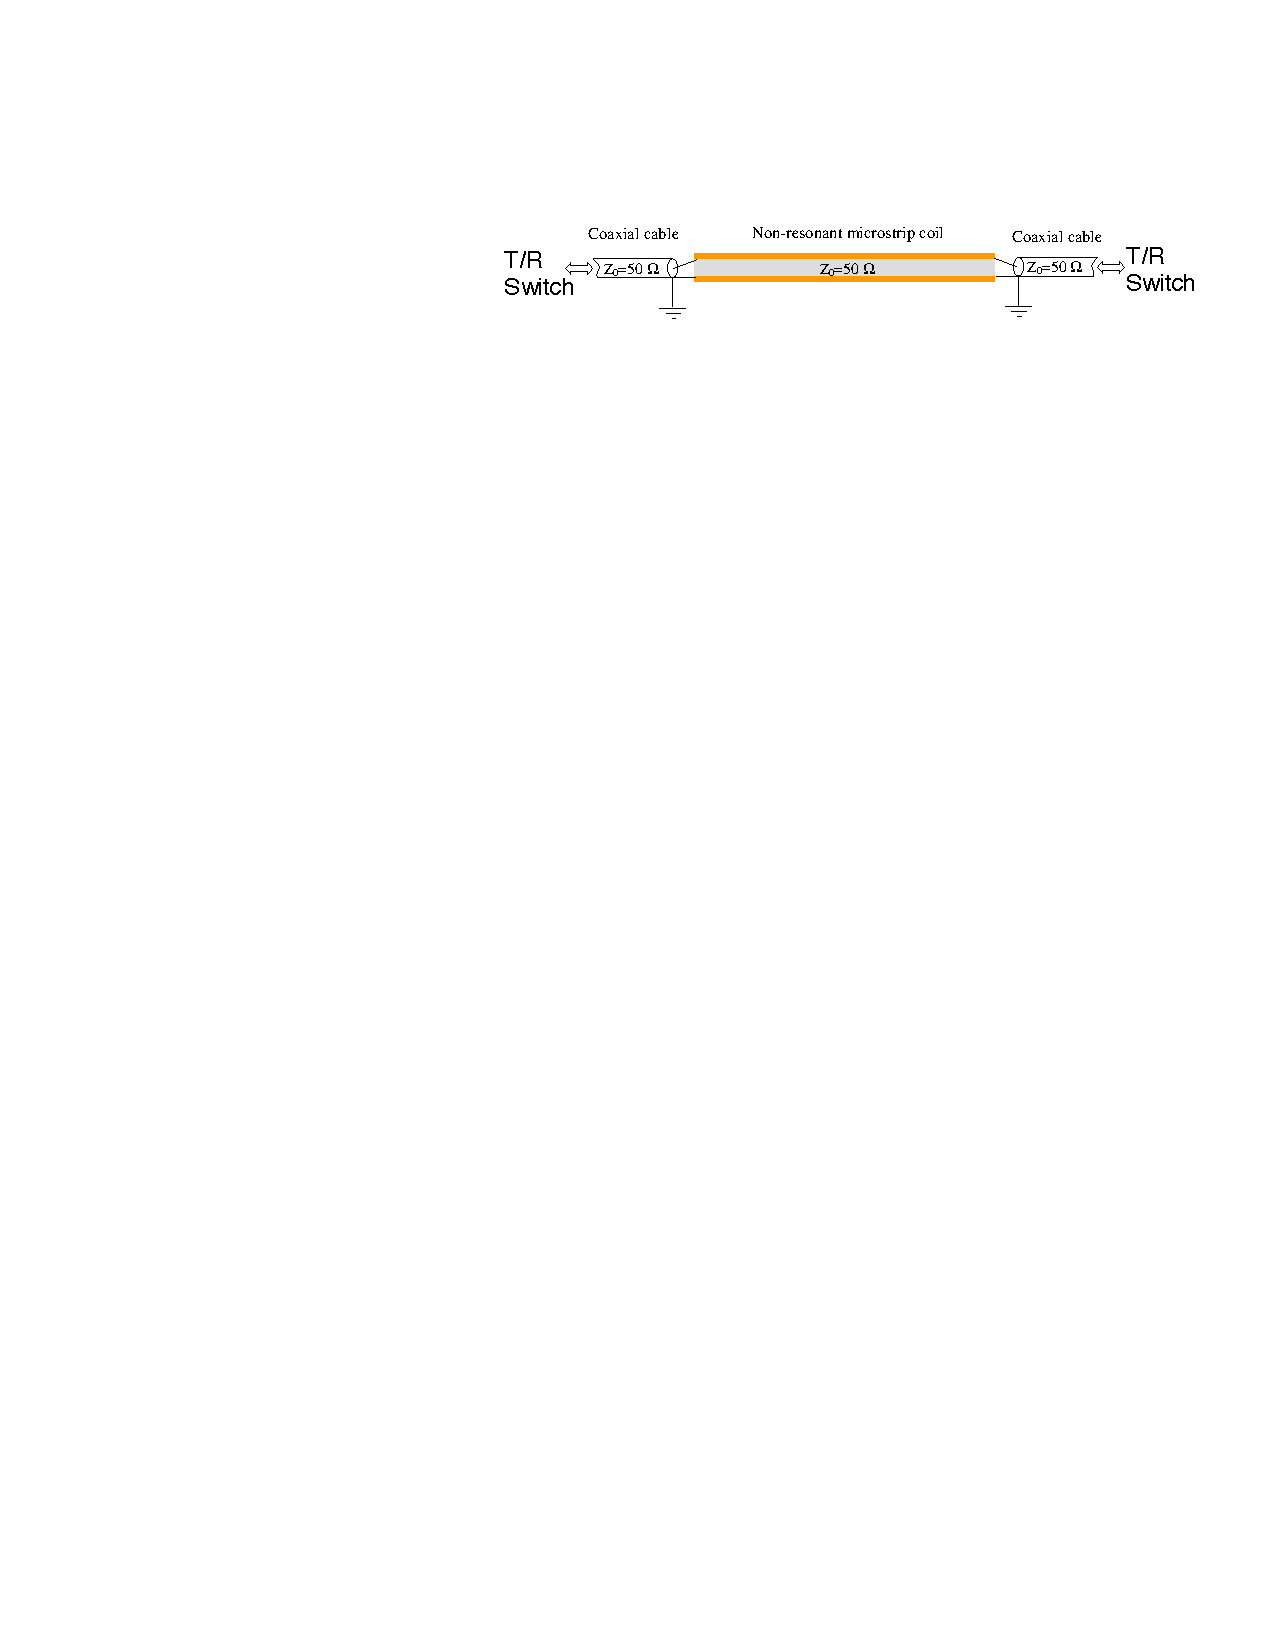
\includegraphics[width=6cm]{Zhang-2008uh-F1}} ;
			\node at (5,0) {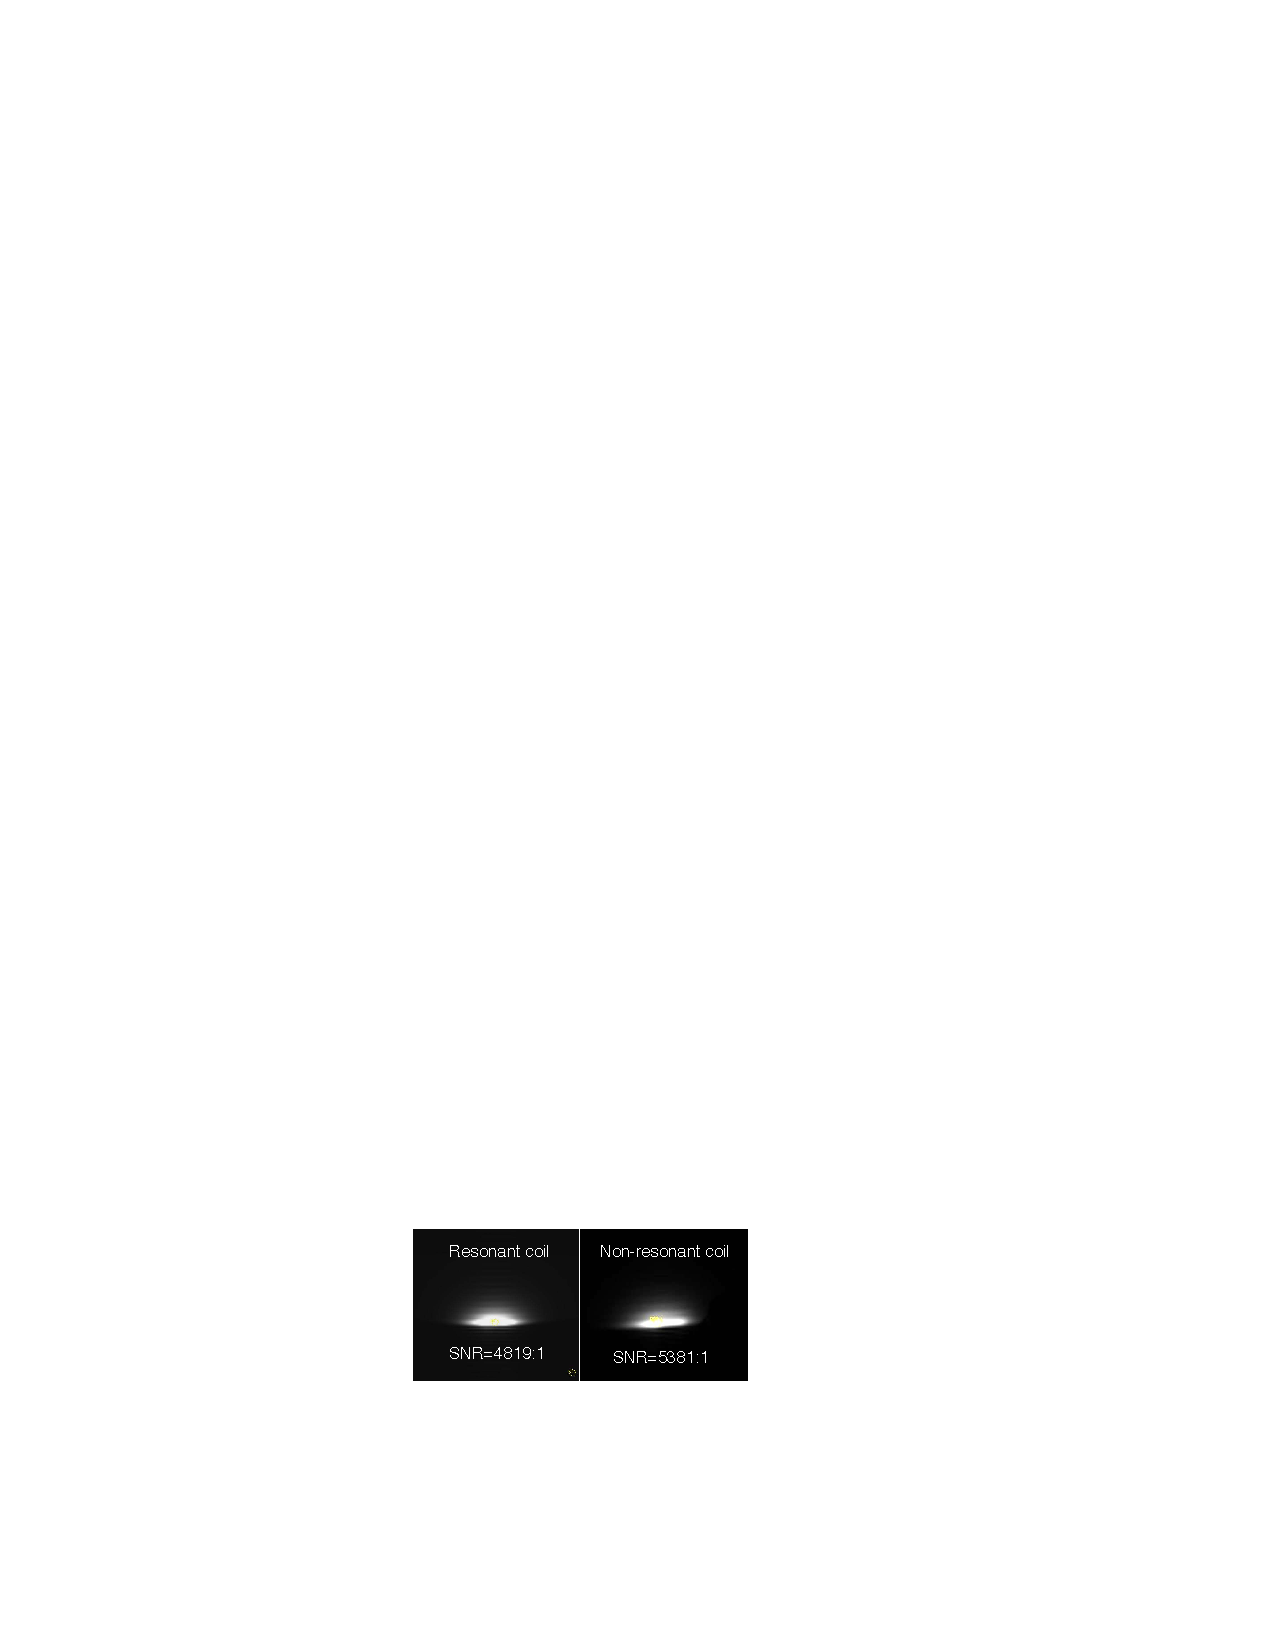
\includegraphics[width=4cm]{Zhang-2008uh-F3}} ;
		\end{tikzpicture}
	\end{center}
	\caption{Non-resonant microstrip detector (left), and MR images obtained
		from a sample of corn oil at 7~T with a resonant and a non-resonant
		microstrip detector. Adapted from \cite{Zhang:2008uh}.}
	\label{fig-Zhang-2008uh}
\end{figure}

Linear non resonant microstrip detectors have been investigated by Zhang
et al \cite{Zhang:2008uh}, who have also performed a direct comparison of
the sensitivity of a microstrip operated in non-resonant and in
standing-wave mode. In a non-resonant system, the spin precession is
coupled into the TEM mode of the transmission line in both directions.
Therefore, Zhang et al used transmit/recieve switches at either end of
the transmission line, and combined the signal power from both before
pre-amplification \cite{Zhang:2009tu}. Interestingly, the SNR from this
setup was found to be the same as in the traditional standing-wave
operation. 

Travelling wave excitation and detection has been considered
as a way to circumvent limitations of high-field full body MRI, where
the dimensions of the sample are comparable to the wavelength of the RF
radiation. In conventional near-field detectors, this leads to uneven
phase and amplitude of the RF signals throughout the sample. Brunner et
al. have demonstrated that MR images with high sensitivity and good
homogeneity can be obtained at 7~T by travelling wave detection
\cite{Brunner:2009ff}. In this case, the conductive bore casing acts as a
cylindrical transmission line, and the \chemical{TE_{01}} mode is excited using
circularly polarised patch antenna near the entrance to the bore. The
possibility to place the detector and excitation structures remotely
from the sample is another advantage of travelling wave systems over
conventional standing wave MR detectors.

 Travelling wave detection has
also been investigated directly in a coaxial cable running vertically
through the bore of a NMR magnet, with the sample taking the place of
the dielectric in the homogeneous area of the magnet \cite{Tang:2011ev},
and a similar design using a planar transmission line has been proposed,
but not yet demonstrated experimentally. A related concept has been
proposed recently by Fratila et al, who directly connected a planar
micro coil between the coaxial transmission line and a matched ohmic
termination \cite{Fratila:2014bv}.

\subsection{Stripline Detectors}
Striplines and microstrips are closely related, 
the main difference being that the
magnetic and electric fields in a stripline are bounded on both sides by
ground planes, in contrast to the one-sided microstrip. Striplines have
been introduced to microwave technology earlier than microstrips, but
are less commonly used in contemporary microwave circuits due to more
complex fabrication. However, they do offer some advantages when used as
NMR detectors. 

Kentgens et al. have built a stripline detector for
micro-NMR on printed circuit board, with the sample replacing the
dielectric on one side of the stripline \cite{vanBentum:2007fd}. A
constriction in the stripline at the location of the sample causes a
concentration of the current, and correspondingly, the RF magnetic
field. A PCB material with a low loss tangent was used to optimise
sensitivity. The stripline was tuned and matched to both the \chemical{^1H} and 
\chemical{^{13}C} frequencies by inserting it as a short to ground at the end of
transmission line resonators made from semirigid coaxial cable. This
arrangement allows \chemical{^1H}--\chemical{^{13}C}  double resonance experiments;
however, no such results were reported \cite{vanBentum:2007fd}. 

The sample volume was about
100~nL, and a mass sensitivity of $10^{13}$ spins/\chemical{\sqrt{Hz}}, or about 0.1
nMol~\chemical{\sqrt{s}} was obtained. It should be noted, however, that this refers
to the single-scan detection limit, and that a more realistic measure of
sensitivity would take into account the delay required for the
acquisition of multiple transients. The $B_1$ homogeneity of the detector
was quite good, at a 810/90 ratio of about 60\%. However, the $B_0$
homogeneity was relatively poor in this initial design. 

A more sophisticated variant was presented by Bart el al
\cite{Bart:2009kc} (cf \fig{fig-Bart-2010wi}). The improved stripline has been designed directly as a
symmetric RF resonator, supporting a $\lambda/2$ standing wave with
current nodes at the ends. A constriction
at the centre of the stripline causes a local increase in magnetic field, and a
concomitant increase in local sensitivity. The resonator is arranged
vertically, parallel to the static magnetic field, thus minimising
susceptibility broadening artefacts. The geometry of the resonator,
including the constriction width, length, and angle of the taper, had
been carefully optimised using finite element computations
\cite{Bart:2009er} for sensitivity and $B_0$ and $B_1$ homogeneity. Bart et al.
showed that the length/width ratio of the constriction is crucial for
sensitivity, and found that ratios between 5 and 10 are optimal. Steep
tapers were found to be preferable in terms of sensitivity, but produce
greater $B_0$ homogeneity artefacts. 

The probe was fabricated by Cu vapour
deposition and subsequent electroplating onto a Si substrate, which
served as a dielectric for the stripline. On one side, the sample
channel is etched into the Si, replacing a part of the dielectric. Ultra
pure, low-conductivity Si is an excellent insulator at room temperature,
and exhibits a low loss tangent. However, it typically carries surface
layer rich in defects, which lead to high dielectric and ohmic losses.
To avoid these, Bart et al. deposited a layer of amorphous silicon
(a-Si) before the metallisation. While this substantially increased the
quality of the resonator, the achieved sensitivity was still about an
order of magnitude less than theoretically predicted. Nonetheless, very
high quality microfluidic NMR spectra have been obtained with 
this system. A limit of detection of $\text{nLOD}_\omega=22.2$~nMol~$\sqrt{s}$ was
demonstrated for the anomeric proton in sucrose in a sample volume of
600~nL, at a spectral resolution of better than 1Hz. 
Bart et al. also
showed that a useful metabolomic spectrum could be obtained from a
sample of human cerebrospinal fluid, even though this required several
hours of acquisition time. 

\begin{figure}
	\begin{center}
		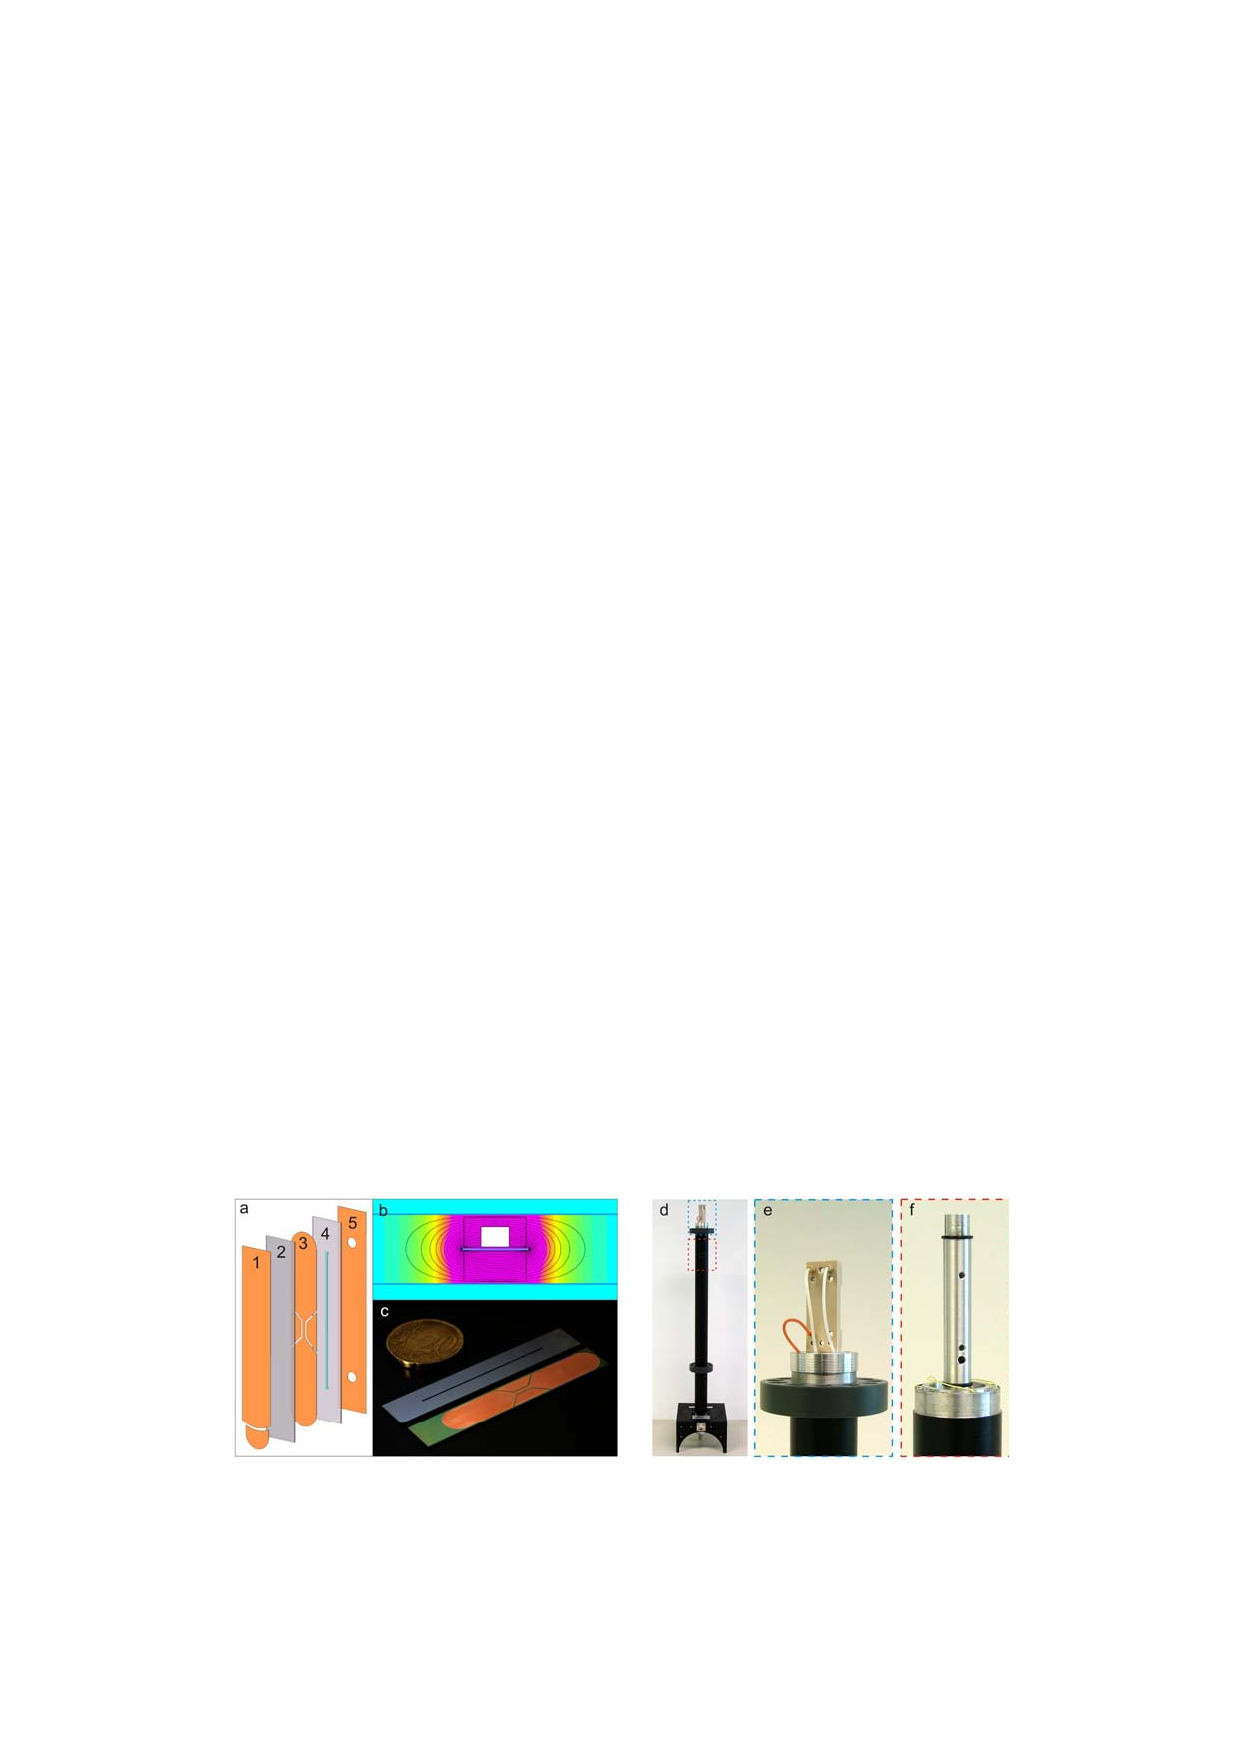
\includegraphics[width=10cm]{Bart-2010wi-F1}
	\end{center}
	\caption{Microfluidic NMR chip and stripline probe. (a) Conductor and 
		dielectric layers of the stripline detector; (b) calculated RF magnetic field distribution;
		(c) photograph of the stripline detector and sample channel; (d-f) NMR flow probe assembly.
		Reprinted with permission from \cite{Bart:2010wi}.
		}
	\label{fig-Bart-2010wi}
\end{figure}


This type of stripline probe has meanwhile
been adapted to a number of interesting applications. The flow-through
probe described by Bart et al has been used for in-line reaction
monitoring \cite{Bart:2010wi}. A stripline resonator similar to the first
one described by van Bentum et al \cite{vanBentum:2008jc} has recently been
used to obtain \chemical{^{75}As} NMR spectra from single crystalline epitaxially
grown films of \chemical{Al_xGa_{(1-x)}As}, in which 5 separate As sites could be
distinguished \cite{Goswami:2014ha}. 

A stripline probe has also been
integrated with a electrochemical conversion assay. In order to
accumulate a sufficient concentration of the electrochemical reaction
products, the EC system was integrated with a solid-phase extraction
column, the elute from which was then fed into the flow-through
stripline NMR probe \cite{Falck:2013kv,Falck:2015eu}. 

An interesting recent
development is the hyphenation of supercritical \chemical{CO_2} chromatography
with NMR detection. SCF chromatography exploits the relatively low
viscosity of SCF solvents, which reduce the back pressure at high flow
rates compared to HPLC systems. This allows higher throughput than
standard HPLC, as well as the separation of molecules that are not
soluble in typical HPLC solvents. The combination of SCFC with NMR
detection would be a natural fit, since the solvent does not produce an
NMR signal. Also, the higher throughput means that potentially larger
amounts of sample can be used and collected, which facilitates NMR
observation. Finally, SCF \chemical{CO_2} is a very low viscosity solvent, which
can have a positive impact on spectral resolution, particularly for
small molecules. However, the direct in-line hyphenation of SCFC with
NMR detection has not yet been reported. A proof of principle has been
given by Tayler et al \cite{Tayler:2015gn}, who used an HPLC storage loop
to collect fractions from SCFC, which were then dissolved in methanol
and injected into a stripline flow probe. Stripline and microstrip
probes offer control over the detailed amplitude and phase distribution
of the RF magnetic field. This opens up many possibilities to integrate
spatial information into the NMR signal collection, which have only
sparely been explored to date. 

Tijssen et al. showed that a tapered
strip line produces a well-defined $B_1$ gradient, and have used this in
order to simultaneously acquire NMR spectra of plugs of different
composition injected one after the other into the sample capillary
\cite{Tijssen:2016hu}. The same system can be used for continuous-flow
reaction monitoring. Tijssen et al also demonstrated that the $B_1$
gradient generated by the tapered stripline can be used to compensate
for B0 inhomogeneities, by acquiring a spatially encoded signal from
which the high-resolution NMR spectrum can be retrieved by data
processing. This possibility may have important applications in
permanent magnet NMR systems. 


\begin{figure}
	\begin{center}
		\begin{tikzpicture}
			%\node at (7.5,0) {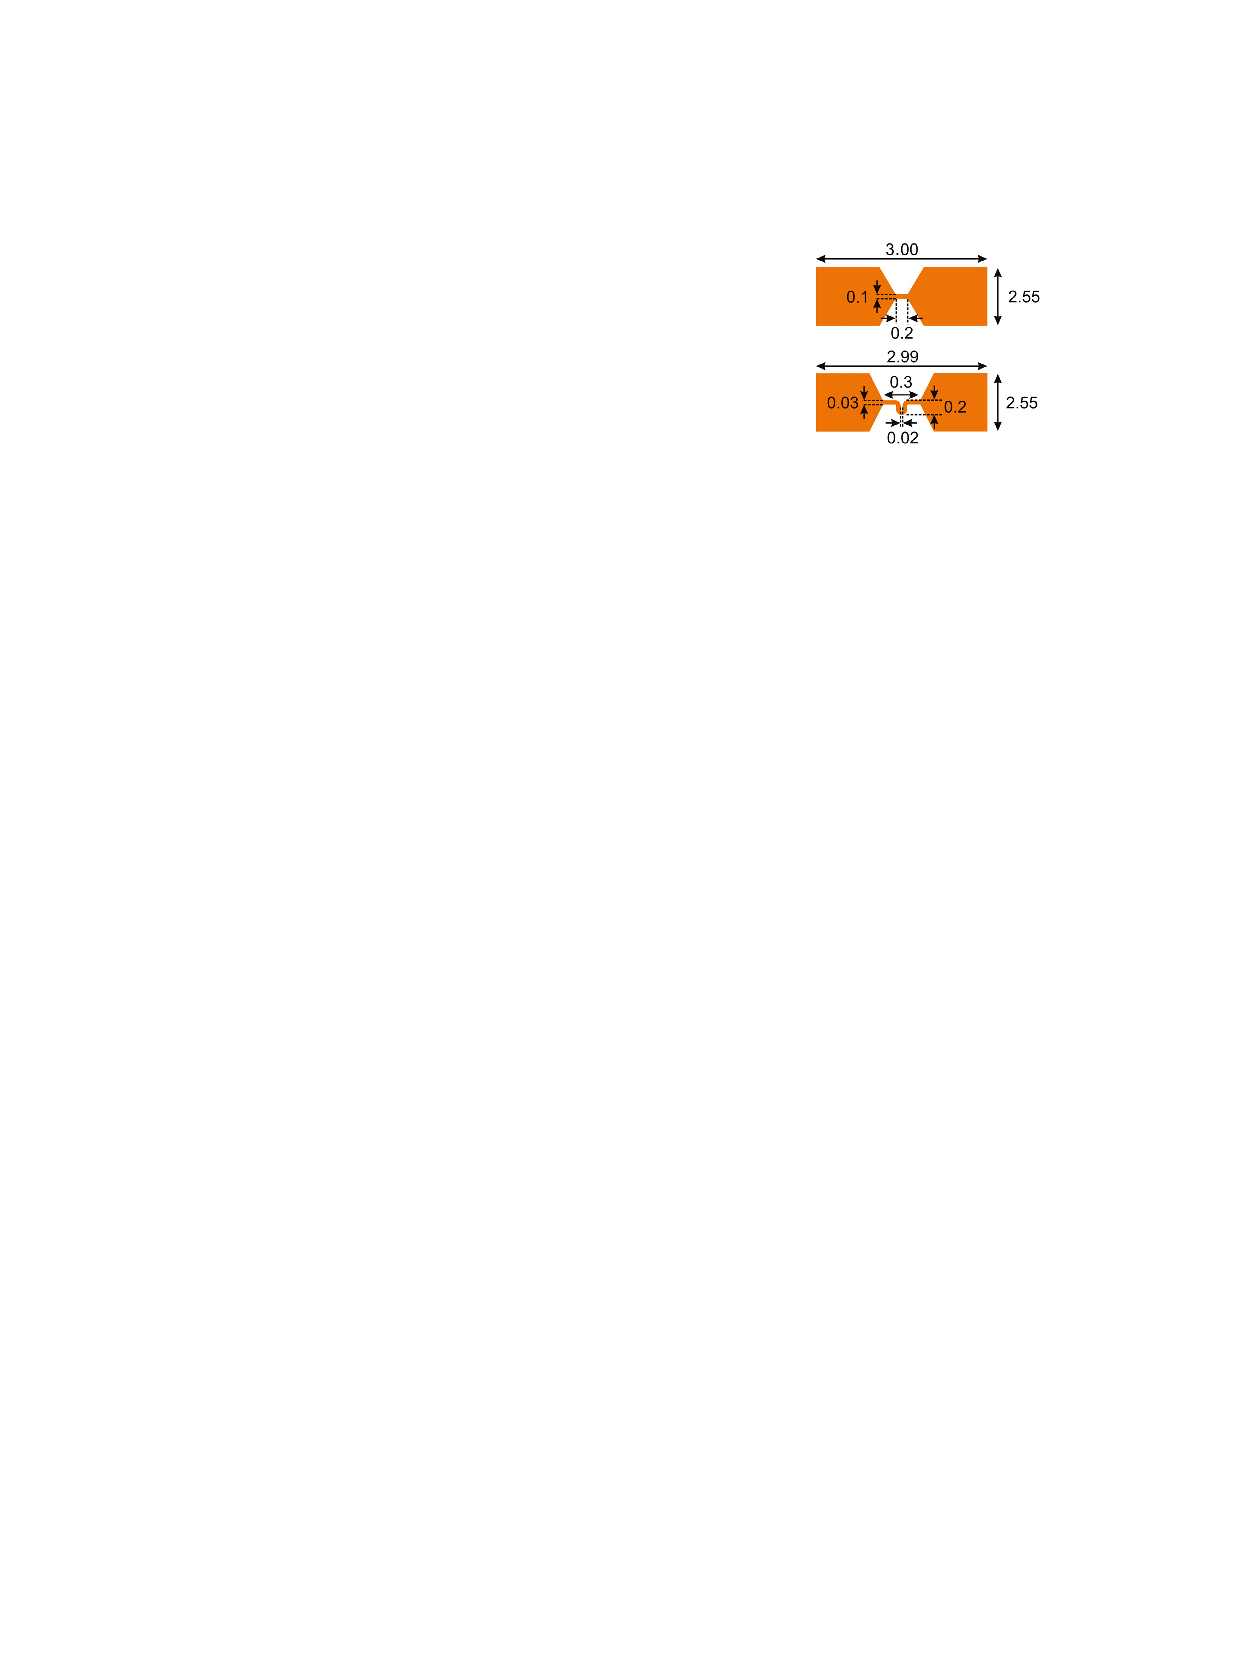
\includegraphics[width=2cm]{Yap-2013ew-F2bc}} ;
			%\node at (4,0) {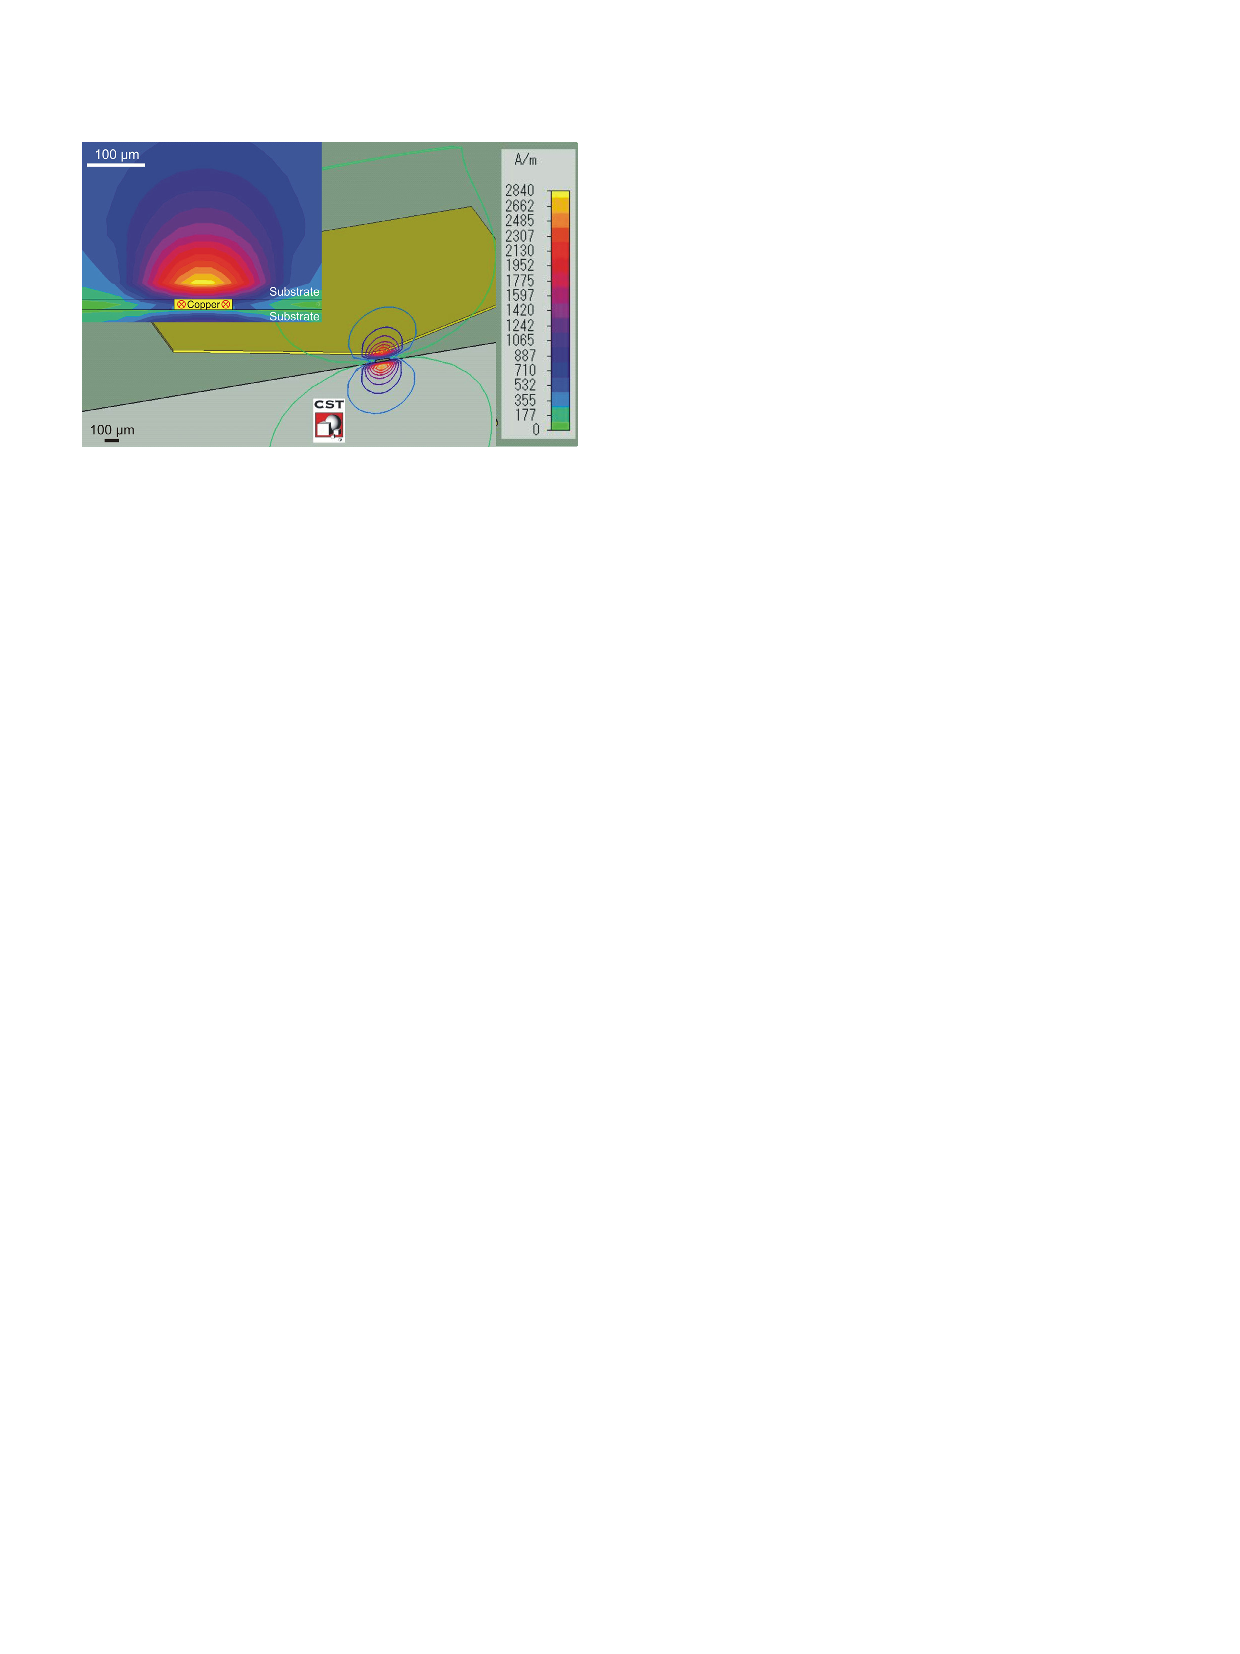
\includegraphics[width=3.5cm]{Yap-2013ew-F4}} ;
			\node at (0,-1.5) {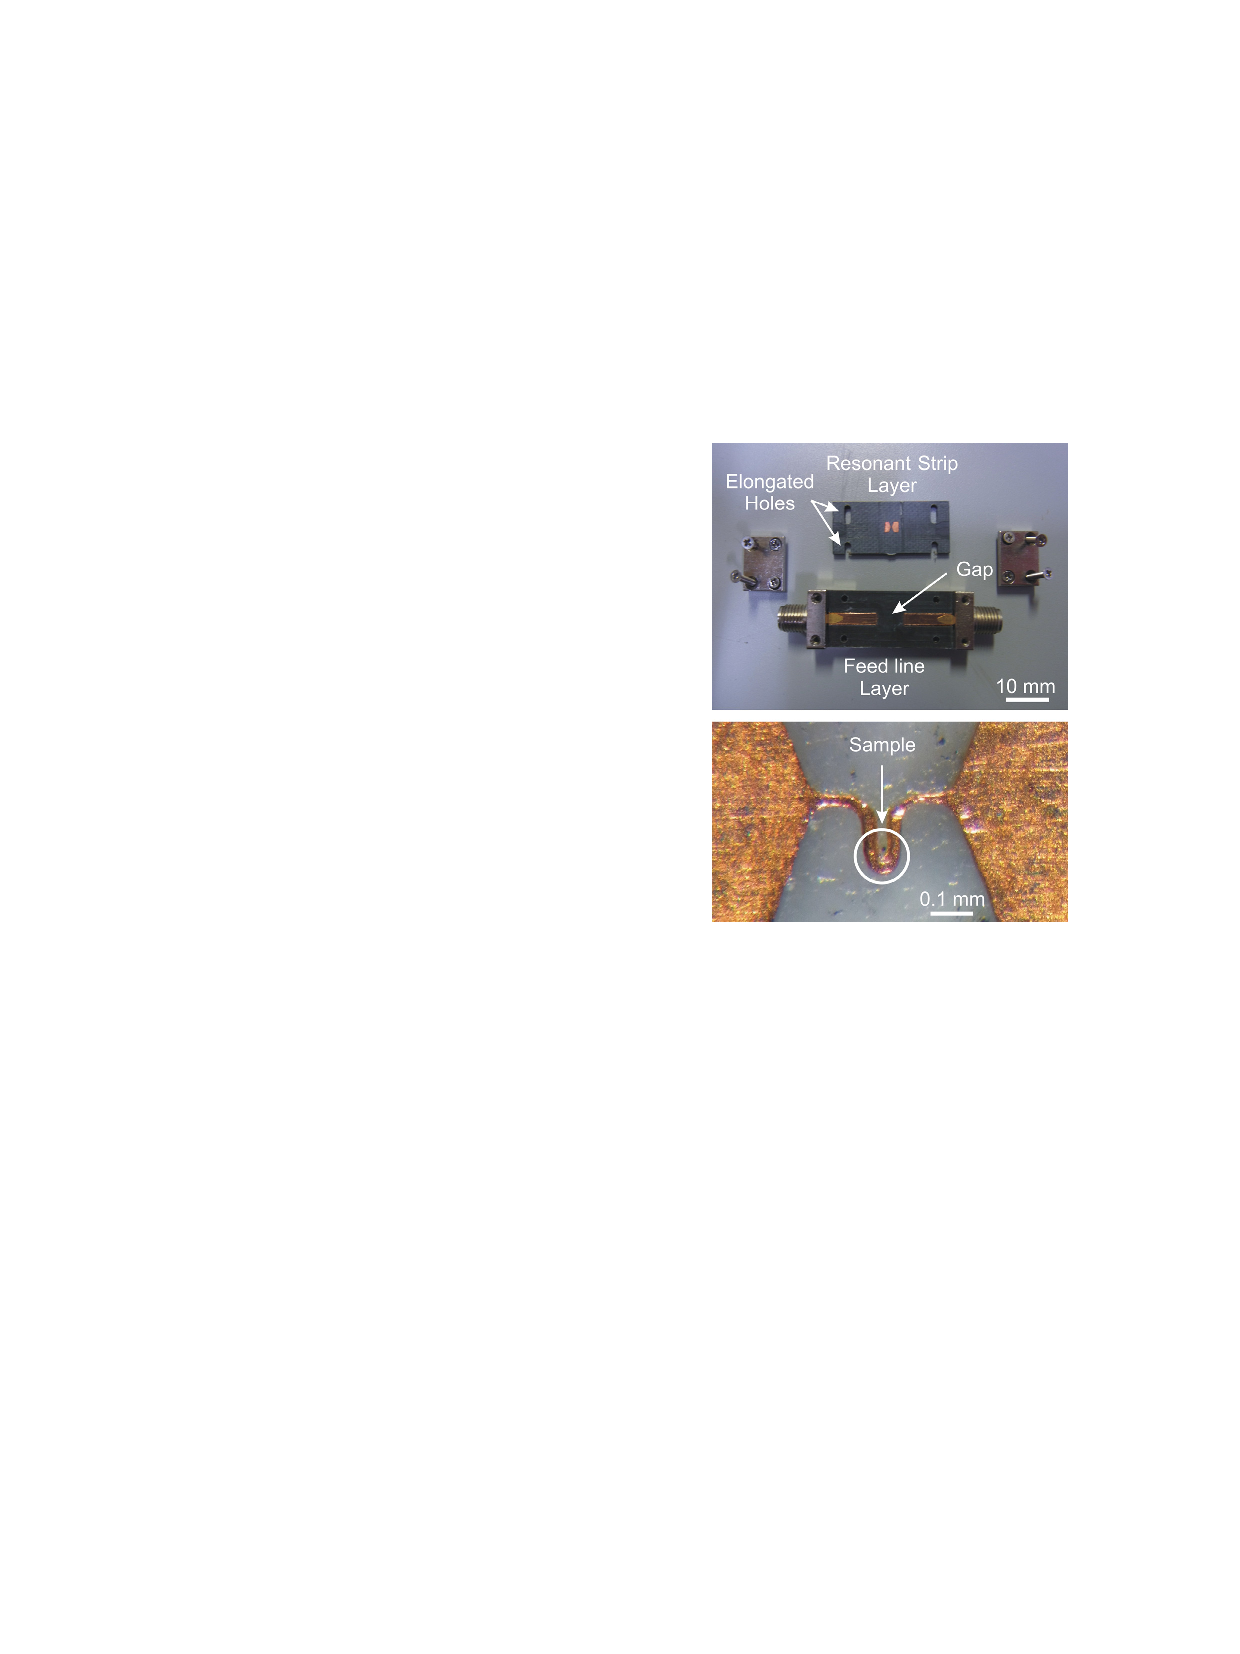
\includegraphics[height=5cm]{Yap-2013ew-F7}} ;
			\node at (6,-1.5) {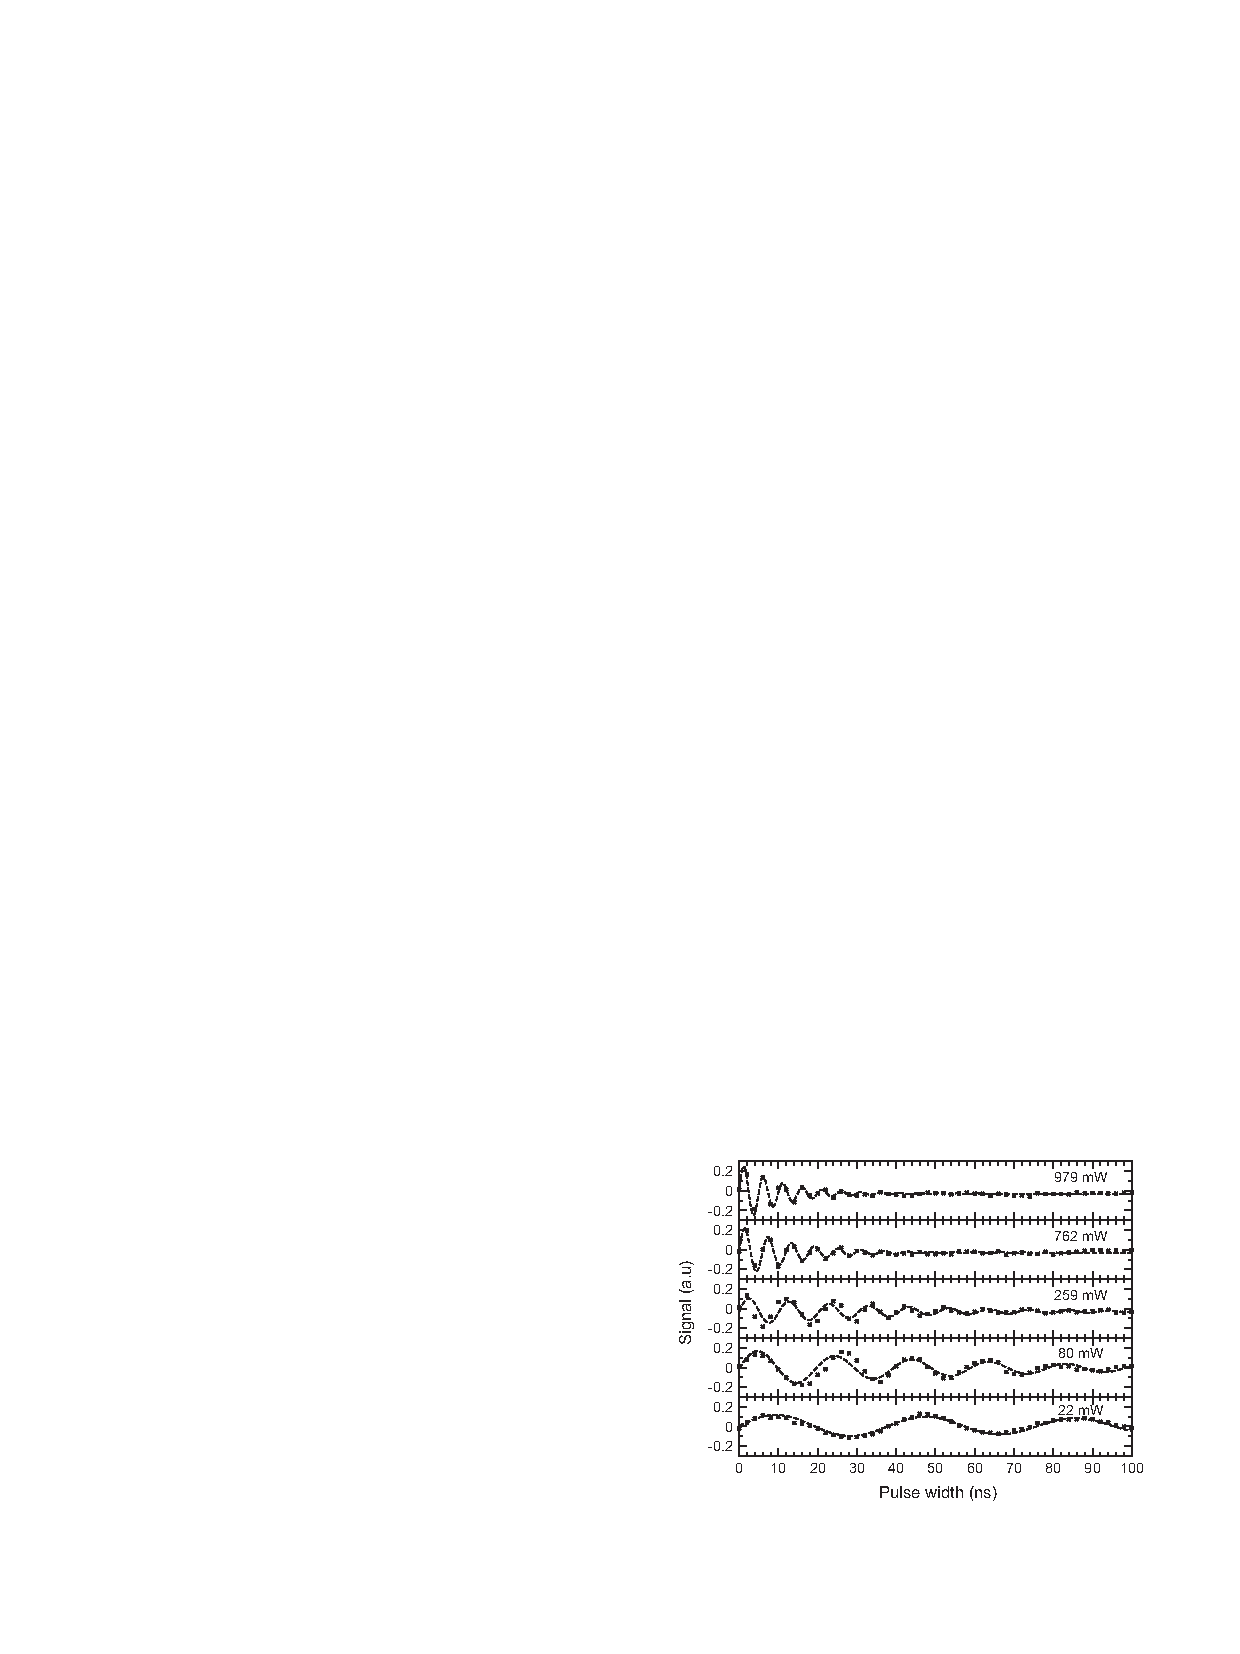
\includegraphics[height=5cm]{Yap-2013ew-F10}} ; 
		\end{tikzpicture}
	\end{center}
	\caption{Stripline resonator for pulsed EPR (left), and nutation diagrams obtained
	with this system (right). Adapted with permission from \cite{Yap:2013ew}.}
	\label{fig-Yap-2013ew}
\end{figure}


Finally, it should be noted that the
stripline design is not only of interest in NMR spectroscopy, but also
in electron paramagnetic resonance. Yap et al. have recently described a
pulsed Ku-band (17 GHz) EPR system based on a micro-stripline resonator (\fig{fig-Yap-2013ew}).
In their design, several variants of the tapered stripline resonator
were explored, including one where the sensitive area is formed by a
narrow, U-shaped turn in the stripline conductor. Using this resonator,
very high sensitivity and Rabi (nutation) frequencies in excess of 210
MHz have been obtained. 

Klotz et al. have used a co-planar stripline
pair to manipulate single electron spins trapped in quantum dots
\cite{Klotz:2011gf}. This type of magnetometer, as well as related systems
based on NV-centre defects in diamond, could become
important as highly sensitive NMR detectors in the future. Waveguide
structures have also been used extensively in the design of probes for
dynamic nuclear polarisation, which require simultaneous irradiation at
NMR and EPR frequencies (see below).


\begin{figure}
	\begin{center}
		\begin{tikzpicture}
			\draw (0,-1.5) node {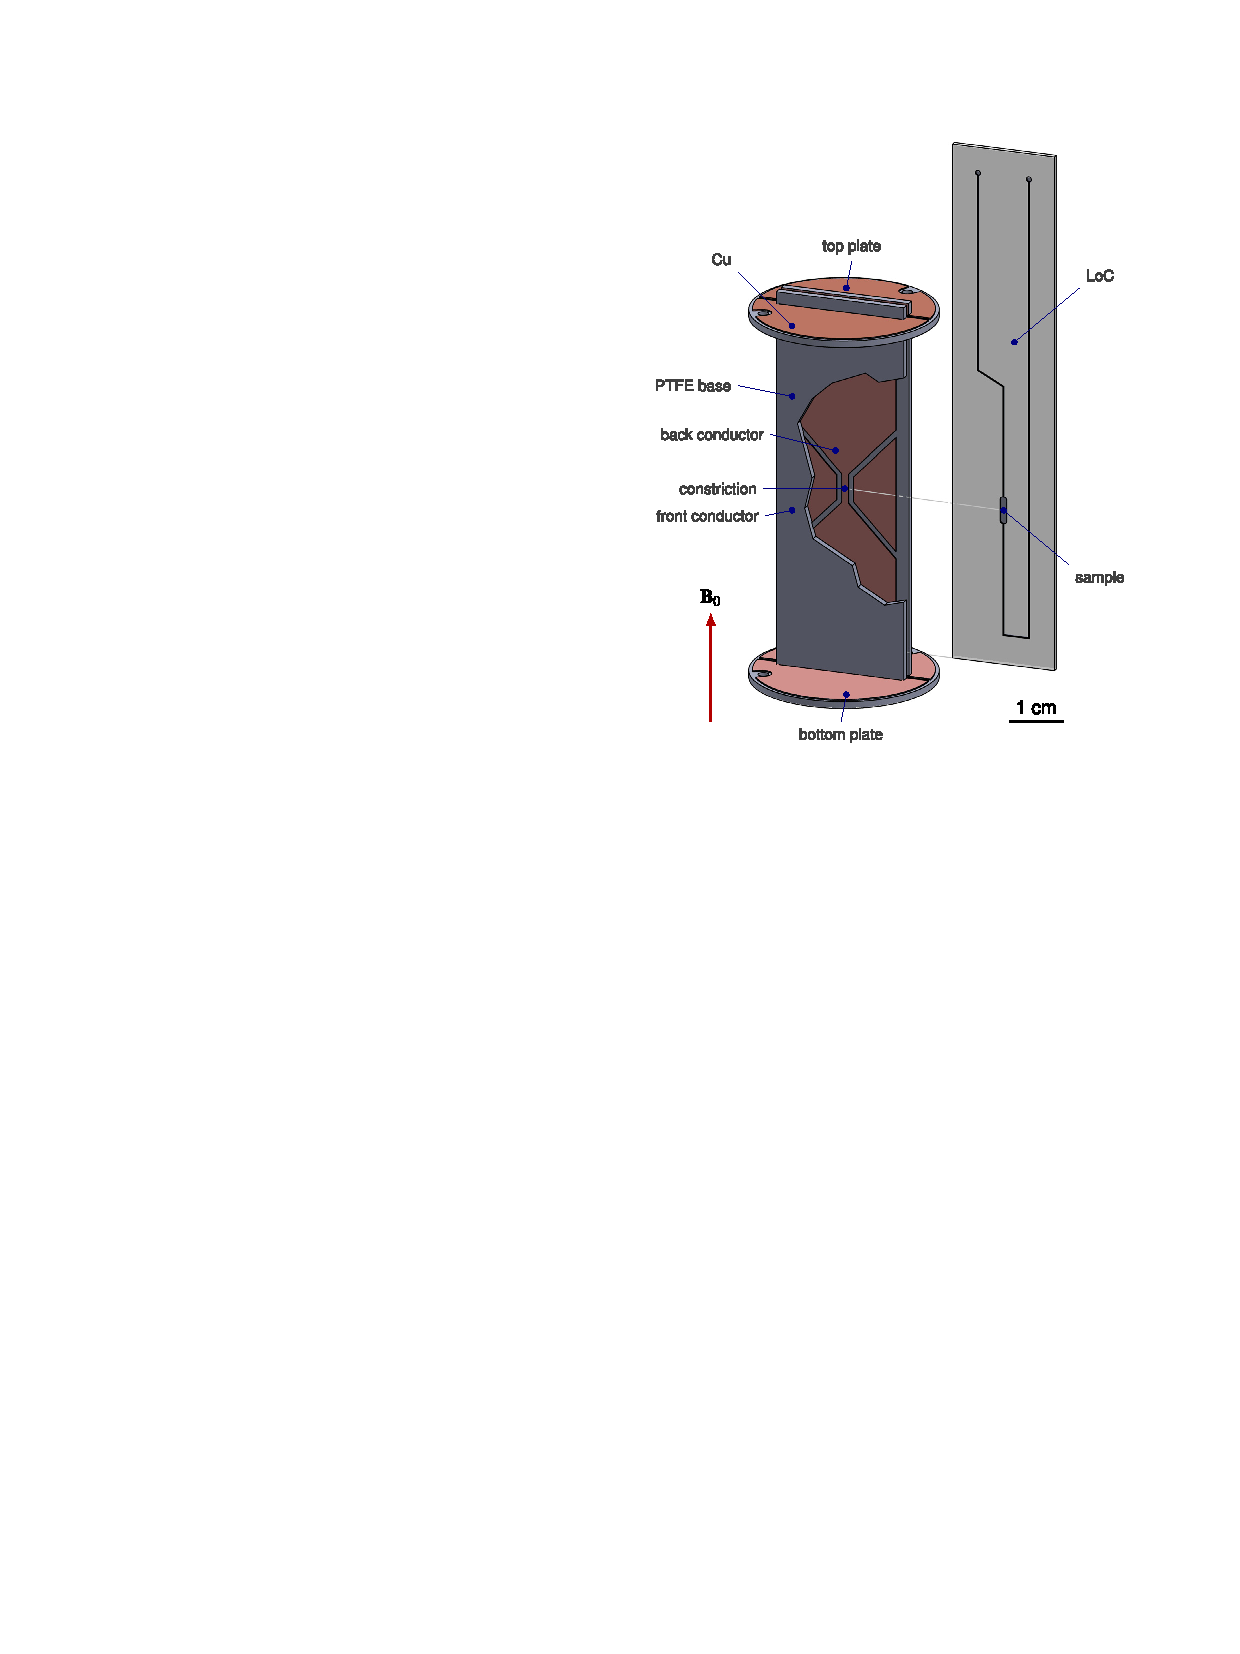
\includegraphics[height=4.5cm]{Finch-2016gv-F2}} ++(-1.5,2.2) node{A};
			\draw (3.5,-0.3)  node {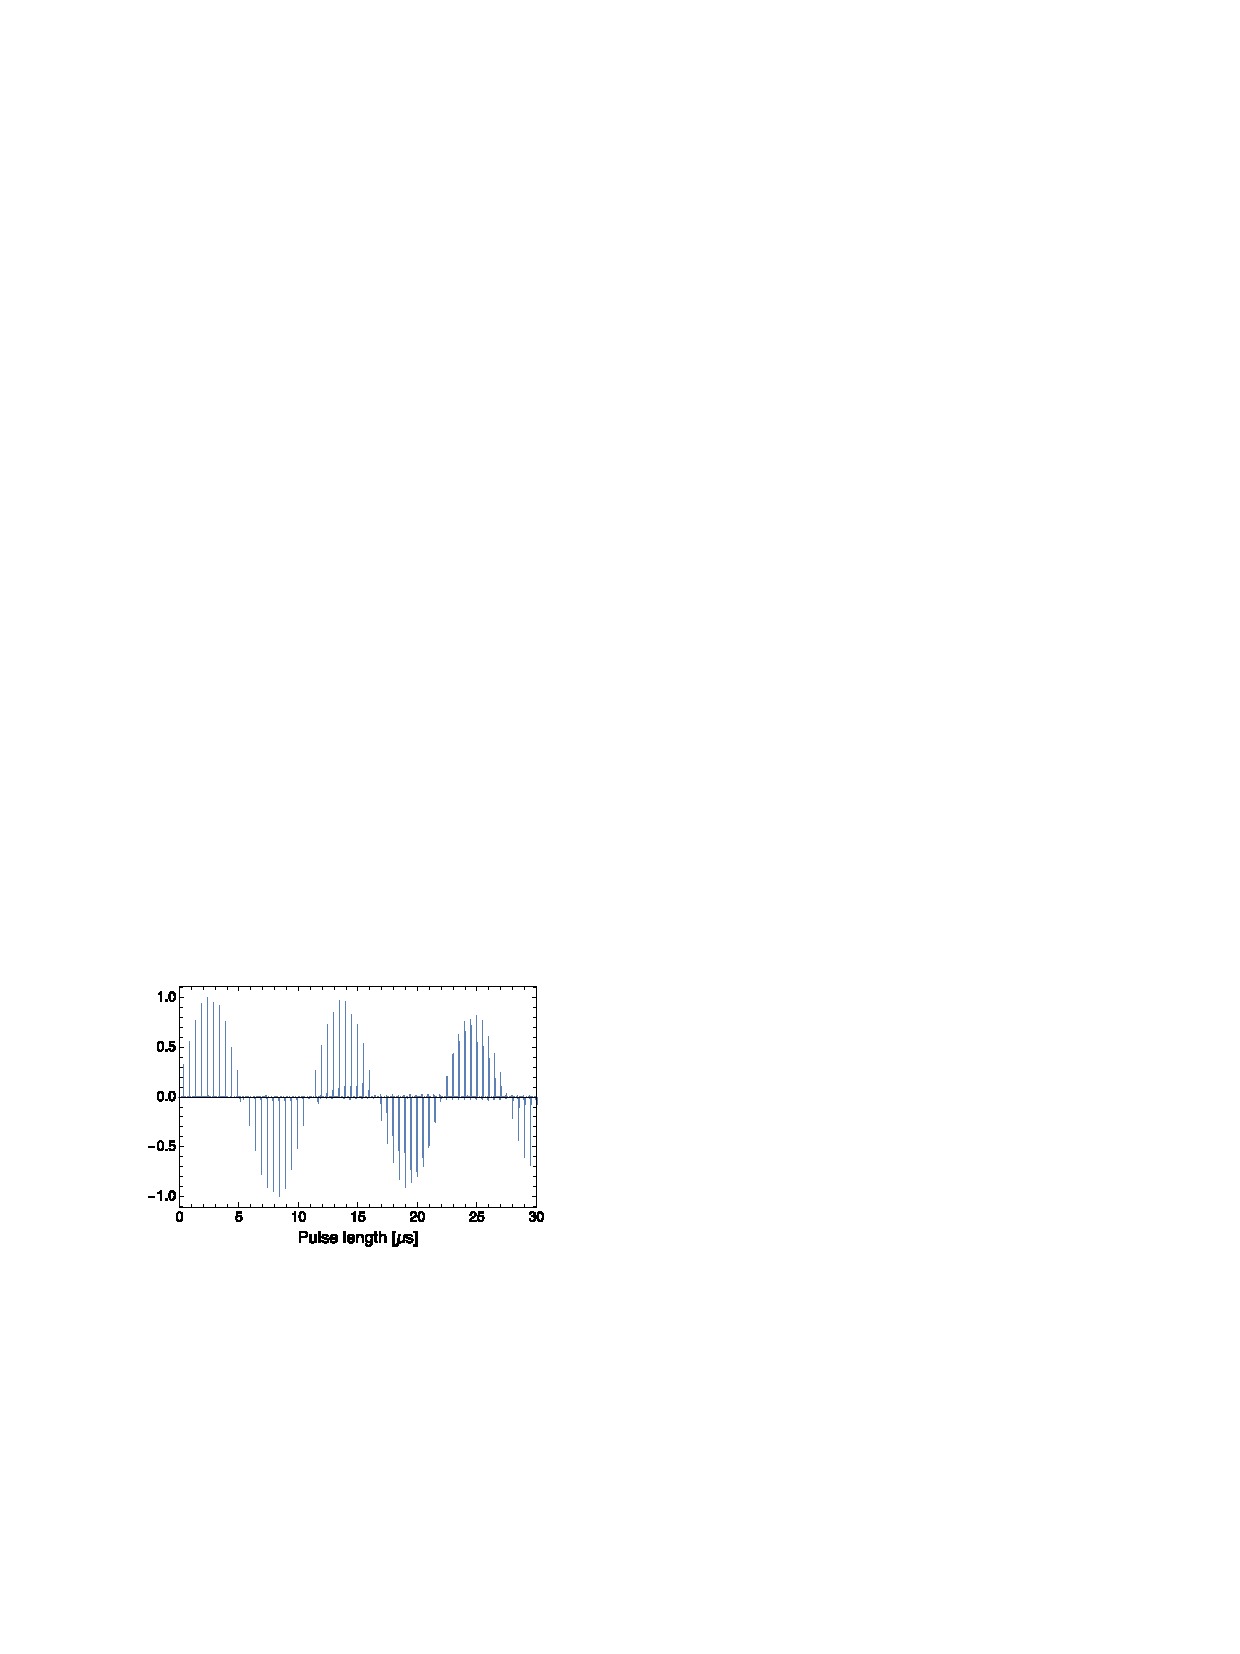
\includegraphics[width=3.cm]{Finch-2016gv-F7d}} ++(-1.8,1) node{B};
			\draw (7.5,-0.3)  node {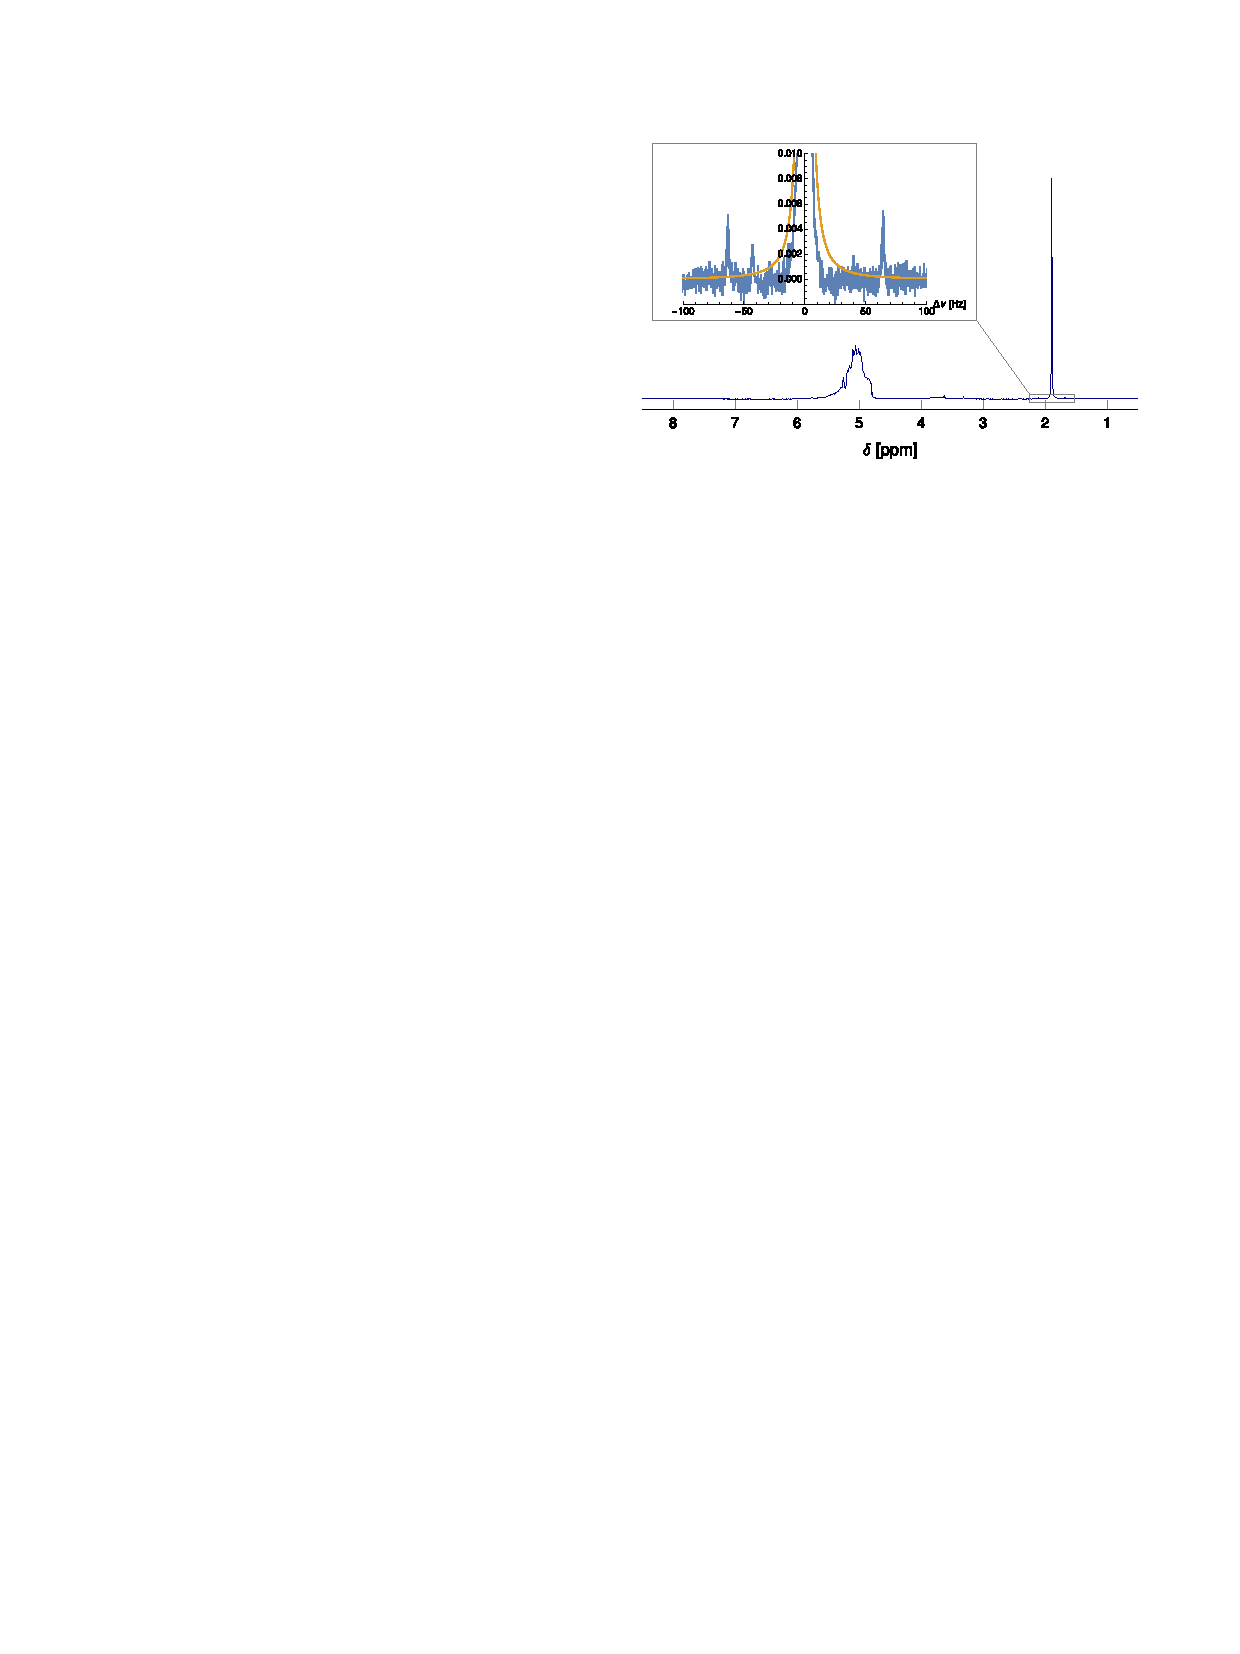
\includegraphics[width=3.cm]{Finch-2016gv-F8}} ++(-1.8,1) node{C};
			\draw (5.5,-2.9) node {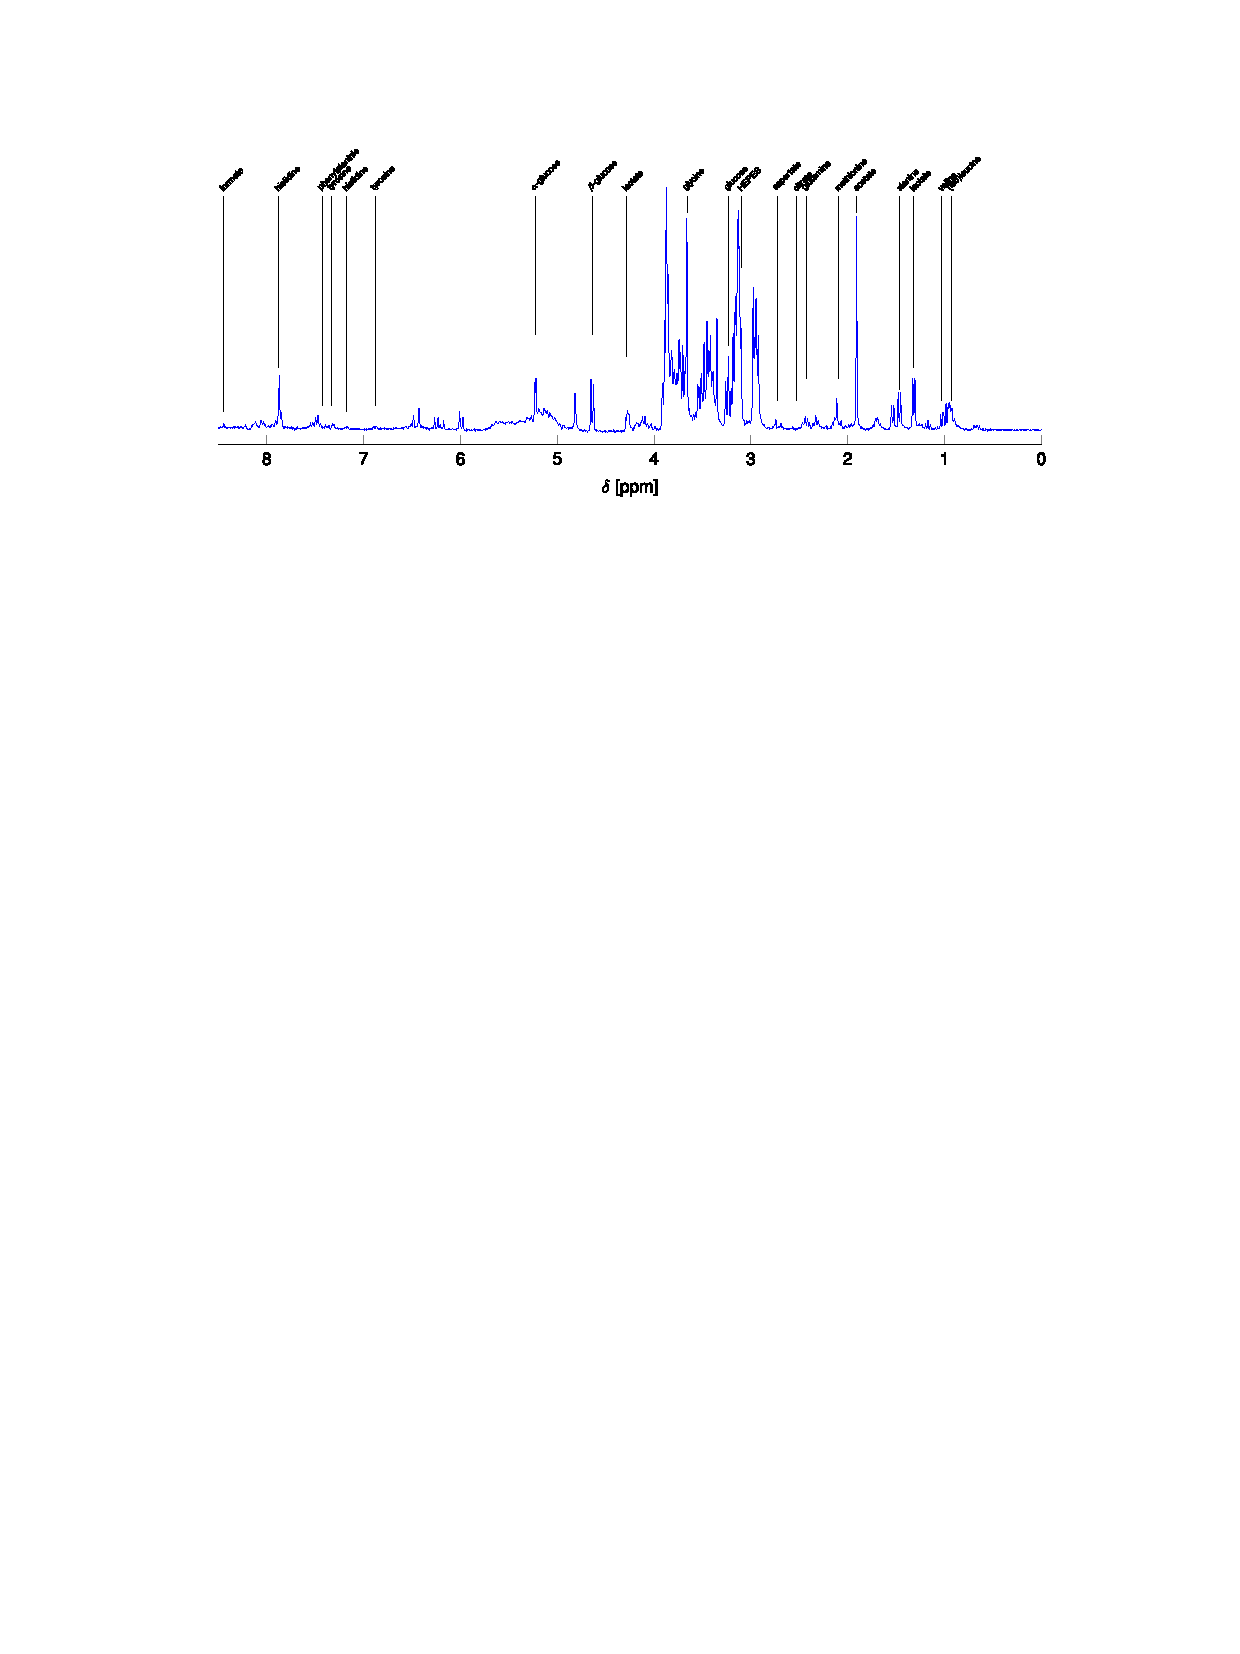
\includegraphics[width=7cm]{Finch-2016gv-F10}} ++(-3.7,1) node{D};
		\end{tikzpicture}
	\end{center}
	\caption{PTL resonator for microfluidic NMR. A: CAD rendering of the resonator and the lab-on-a-chip device; B: experimental nutation curve at 10~W; C: 150 mM acetate in \chemical{H_2O} spectrum demonstrating excellent baseline resolution; D: \chemical{^1H} spectrum of 2 µl of cell growth medium containing 20~mM glucose, and less than 1~mM concentrations of various amino acids. The spectrum was acquired in about 20 min. Adapted with permission from \cite{Finch:2016gv}.}
	\label{fig-Finch-2016gv}
\end{figure}


\subsection{Parallel Plate Transmission Lines}\label{parallel-plate-transmission-lines}

Parallel plate transmission lines (PTL), comprised of two parallel
conductors of equal width, share some of the characteristics of both
stripline and microstrip waveguides. In particular for large $w/h$ ratios,
the electric field is largely contained in the dielectric space between
the conductors. However, there is some spillover into the surrounding
space, and the magnetic field lines are not contained, but loop around
each conductor, as shown in \fig{fig:cross-sections}D. Like microstrips, and in contrast
to striplines, PTL do not support a pure TEM mode in general, due to the
difference in dielectric constant between the dielectric material and
the surrounding air. In the context of magnetic resonance detectors, the
PTL geometry is a natural fit with planar samples, and it is somewhat
surprising that it has not been exploited more extensively to date.

Jasisnski et al have built a micro imaging NMR probe head using a
resonator based on a PTL of 5 mm length and 0.3 mm width
\cite{Jasinski:2012cn}. The $w/h$ ratio had been optimised using
two-dimensional finite element calculations; it was found that $w/h$
values in the vicinity of unity provided a good compromise between RF
homogeneity, filling factor, and sensitivity. The PTL was tuned and
matched to a 50 Ohm coaxial cable, giving an unloaded Q factor of 120,
in good agreement with the finite element simulations. The resonator was
placed in a magnetic field of 11.7~T, with the magnetic field direction
normal to the conductor planes. High quality images of $24 \times 24 \times 300$~\chemical{\mu m}
resolution on $128\times 128$ points could be obtained  in
about 45 minutes. 

A similar detector was built by Finch et al
\cite{Finch:2016gv} for microfluidic NMR spectroscopy.
Their geometry was an adaptation of the stripline
probe proposed by Bart et al. \cite{Bart:2009kc}, consisting of a half-wave
resonator with the waveguide axis parallel to the magnetic field, and a
constriction at the location of the sample (cf.~\fig{fig-Finch-2016gv}). Unlike earlier
microfluidic NMR probes, which used fixed capillaries requiring
fluidic sample connections, the probe by Finch et al was designed to
accommodate a wide range of lab-on-a-chip devices manufactured from PMMA
sheet material by either by hot embossing, or by inexpensive rapid
prototyping techniques based on a digital laser cutting system. 

Starting
from a requirement of a sample chamber volume of 2 µl, Finch et al. used
a numerical search algorithm in combination with a 3D finite element
model of the resonator to optimise simultaneously the probe chamber
dimensions (width $\times$ length), and the corresponding dimensions of the
constriction in the resonator. The optimisation was balanced between the
conflicting targets of high sensitivity and RF homogeneity, resulting in
a compromise design. This probe achieved a frequency-domain limit of
detection of $\text{nLOD}_\omega = 1.57\;\mathrm{nMol \sqrt{s}}$ (based on signal averaging over
multiple transients), at a line width of 1.78 Hz (at 7 T). Importantly,
the line widths at 0.5\% and 0.1\% height were inside of a Lorentzian
line with the same half-width (\fig{fig-Finch-2016gv}C). This baseline resolution is of particular
importance in metabolomic studies \cite{pan2007cac,Zhang:2010kf}, where
signals of widely differing intensity appear, and broad feet from strong
lines can obscure weaker signals. 

\subsection{Applications in Solid State Physics}

Planar
waveguide structures have been used extensively in solid state physics,
including in experiments that relate directly or indirectly to magnetic
resonance. For example, Yusa et al. have demonstrated the detection of
nuclear spin states in GaAs by subtle effects of the nuclear magnetism
on the conduction of photo-induced charge carriers \cite{Yusa:2005iy} (cf
also \cite{Tycko:2005kj}). This allowed the detection of as few as $10^8$
nuclear spins, which is a remarkable achievement even at the
experimental temperature of 100 mK. 

Conducting microstrips have been
deposited on top of a ferromagnetic layers in order to obtain broadband
ferromagnetic resonance signals. In this way, the magnetic properties of
thin film structures can be studied by inductive microwave spectroscopy
\cite{Kostylev:2009ia,Kostylev:2010fy}. Similar techniques using optical
detection have been described, as well \cite{Keatley:2005by}. 


\subsection{Waveguides for Dynamic Nuclear Polarisation}
While optimised detector
geometries mitigate the inherently poor sensitivity of the NMR
experiment, they do not ultimately address its root cause: the magnetic
polarisation of nuclear spins is minuscule (of the order of 1 spin in $10^5$),
even at the highest practical magnetic fields. Sample cooling helps to
an extent, but is undesirable for many systems, in particular
in biology. 

Several methods are known to temporarily increase the
nuclear polarisation above the thermodynamic equilibrium value,
including parahydrogen-induced polarisation, optical pumping, and
dynamic nuclear polarisation (DNP). Each of these has its
merits and limitations. Among them, DNP is of most interest in the
present context, because it places special requirements on the resonator
structure surrounding the sample. 

DNP transfers polarisation from the
electron to the nuclear spins by cross-relaxation. A radical
species needs to be present in the sample, with suitable electron spin
relaxation times to make the transfer feasible. 
Stable nitroxide radicals are commonly used for this
purpose. DNP requires saturation, or at least significant perturbation,
of the electron spin temperature by microwave irradiation. At typical
NMR magnetic fields, this involves microwave frequencies up to several
hundred GHz. Transporting microwave power in this part of the spectrum
requires carefully designed waveguide structures. DNP tends to be most
efficient in the solid state, and at cryogenic temperatures.

This has led to the development of dissolution-DNP techniques
\cite{ArdenkjaerLarsen:2016jq}, in which the sample is first irradiated with microwaves 
at liquid He temperature or somewhat below for about an hour or
so, then rapidly dissolved in a hot solvent, to be transferred to
an NMR magnet for spectroscopy, or injected into a live subject inside an MRI
scanner for imaging \cite{Brindle:2011hu}. 

The dissolution DNP technique does not lend itself to small scale applications,
due to the experimental overhead; relatively large (ml) volumes of 
hyperpolarised materials are produced in a batch process, with polarisation
life times of only a few minutes at best.

At small enough scale, it is possible to avoid the
dissolution and the transfer step, and rapidly melt the sample in-situ
after microwave irradiation by means of either an electric heater or
exposure to a hot gas. This has been achieved recently by Sharma et al.
\cite{Sharma:2015ce}. A capillary of 360 $\mu$m outer diameter is moved
between three regions inside an NMR magnet: a cold region at 77~K, where
the sample is irradiated with microwaves, a hot region, where the
capillary is exposed to a stream of warm nitrogen gas, and an NMR
region, where the NMR spectrum is measured using a stripline resonator.

\begin{figure}
	\begin{center}
		\begin{tikzpicture}
			\draw (0,0) node {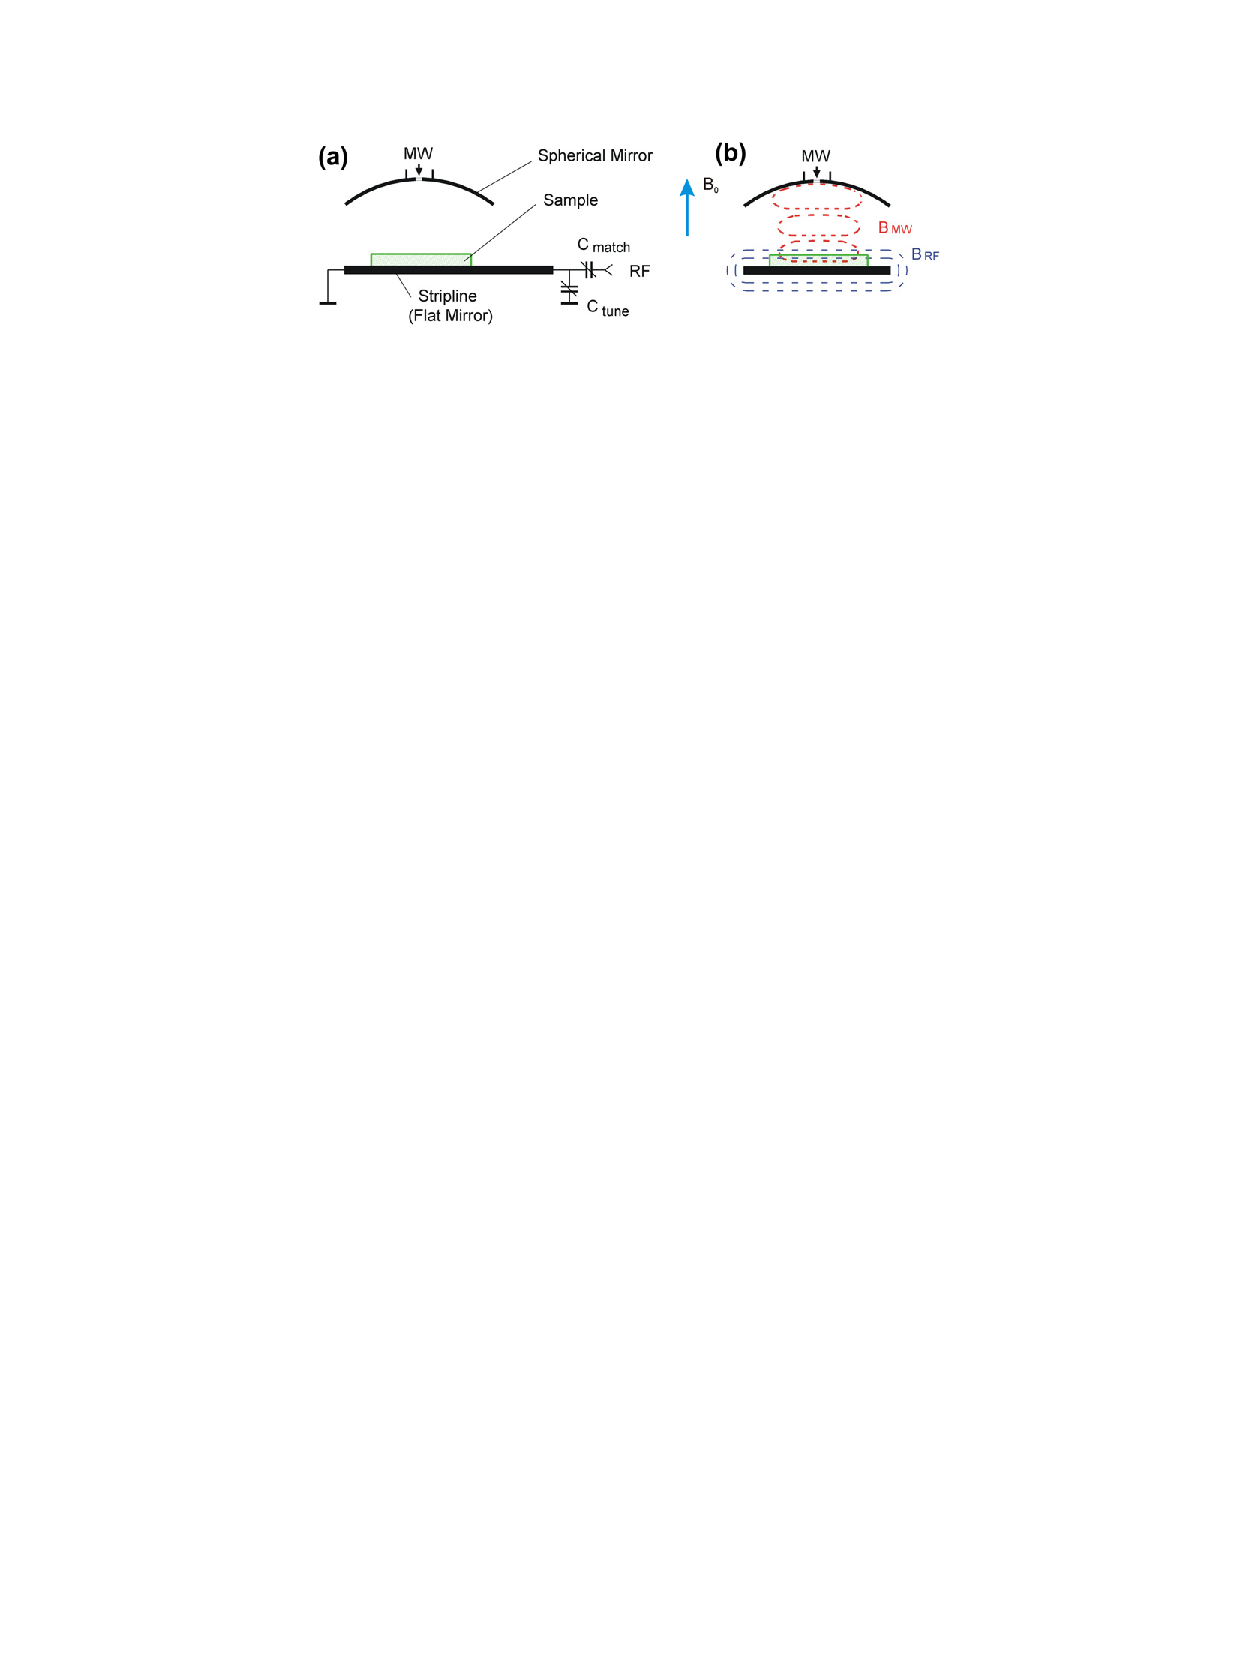
\includegraphics[width=5cm]{Denysenkov-2012jy-F1}} ++(-1.5,1) node{};
			\draw (3.5,0)  node {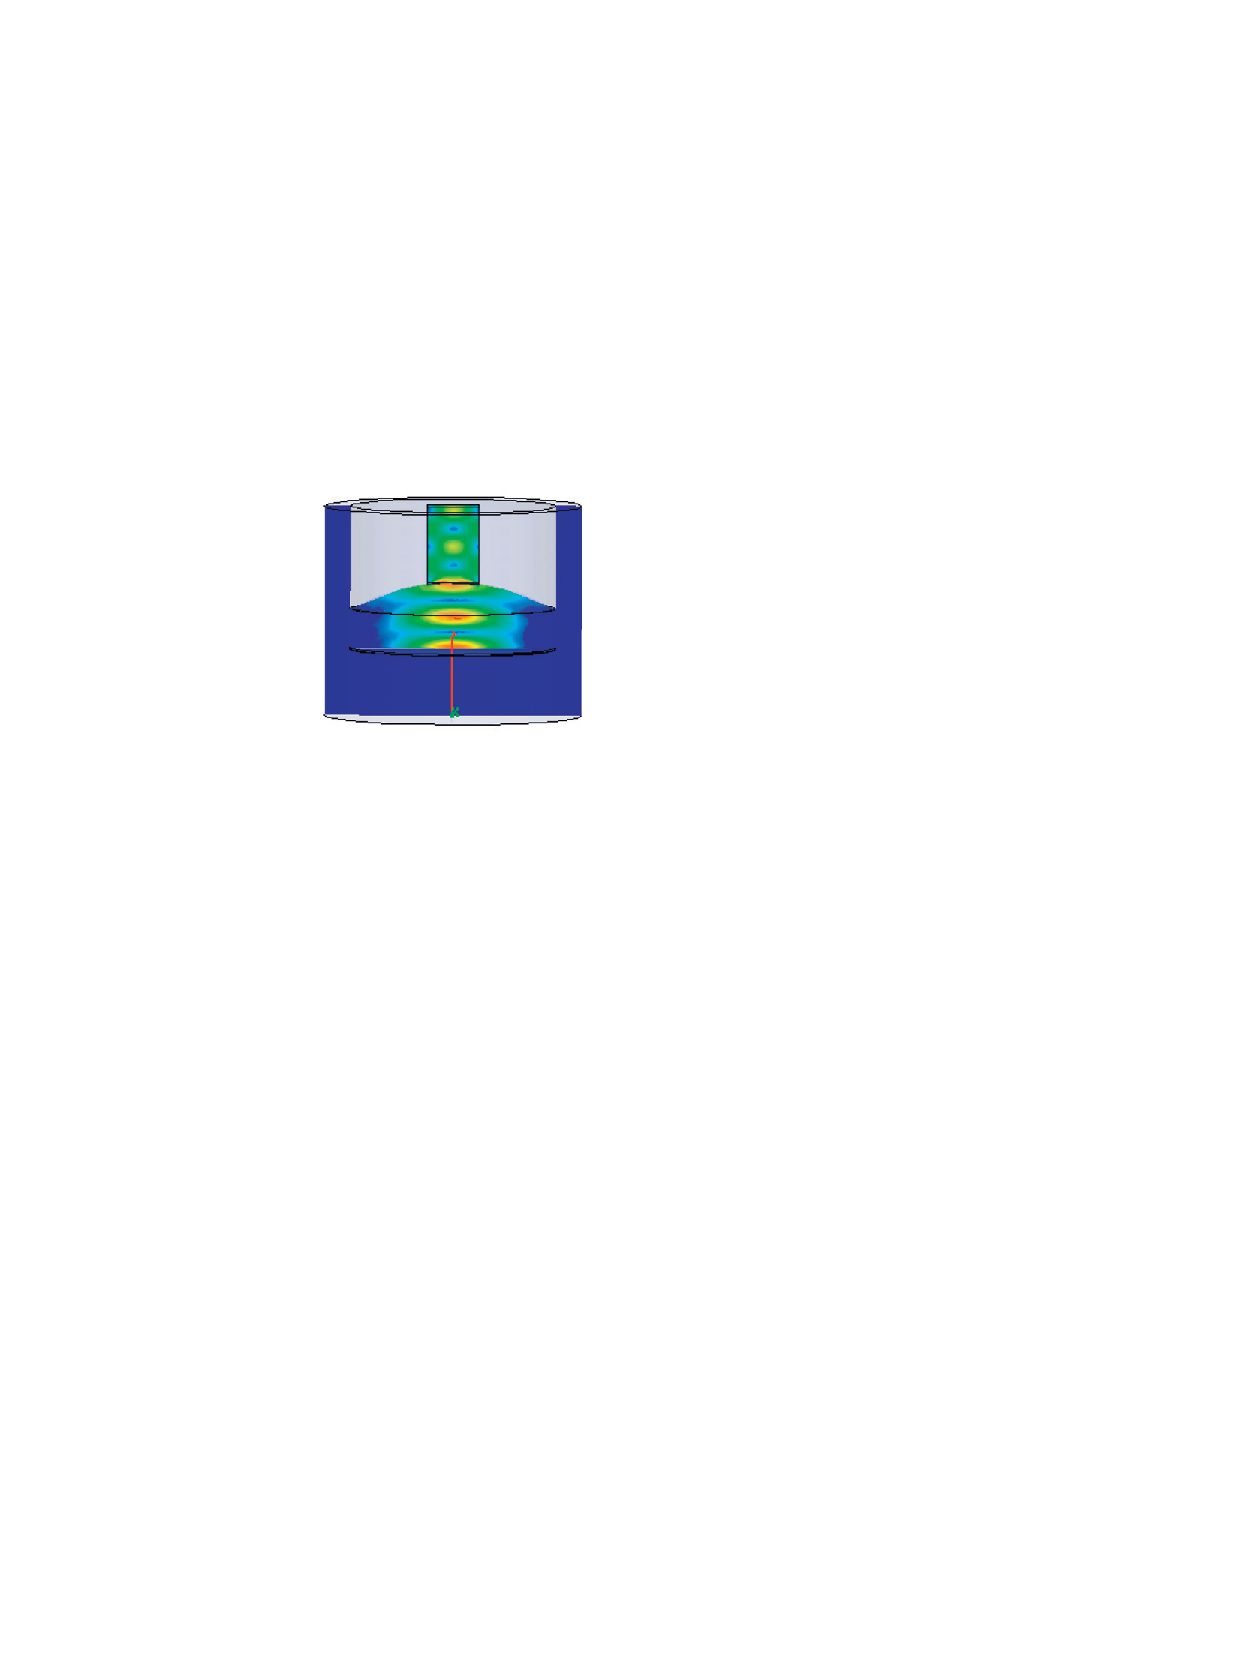
\includegraphics[width=2.cm]{Denysenkov-2012jy-F2a}} ++(-1.8,1) node{};
			\draw (6.5,0)  node {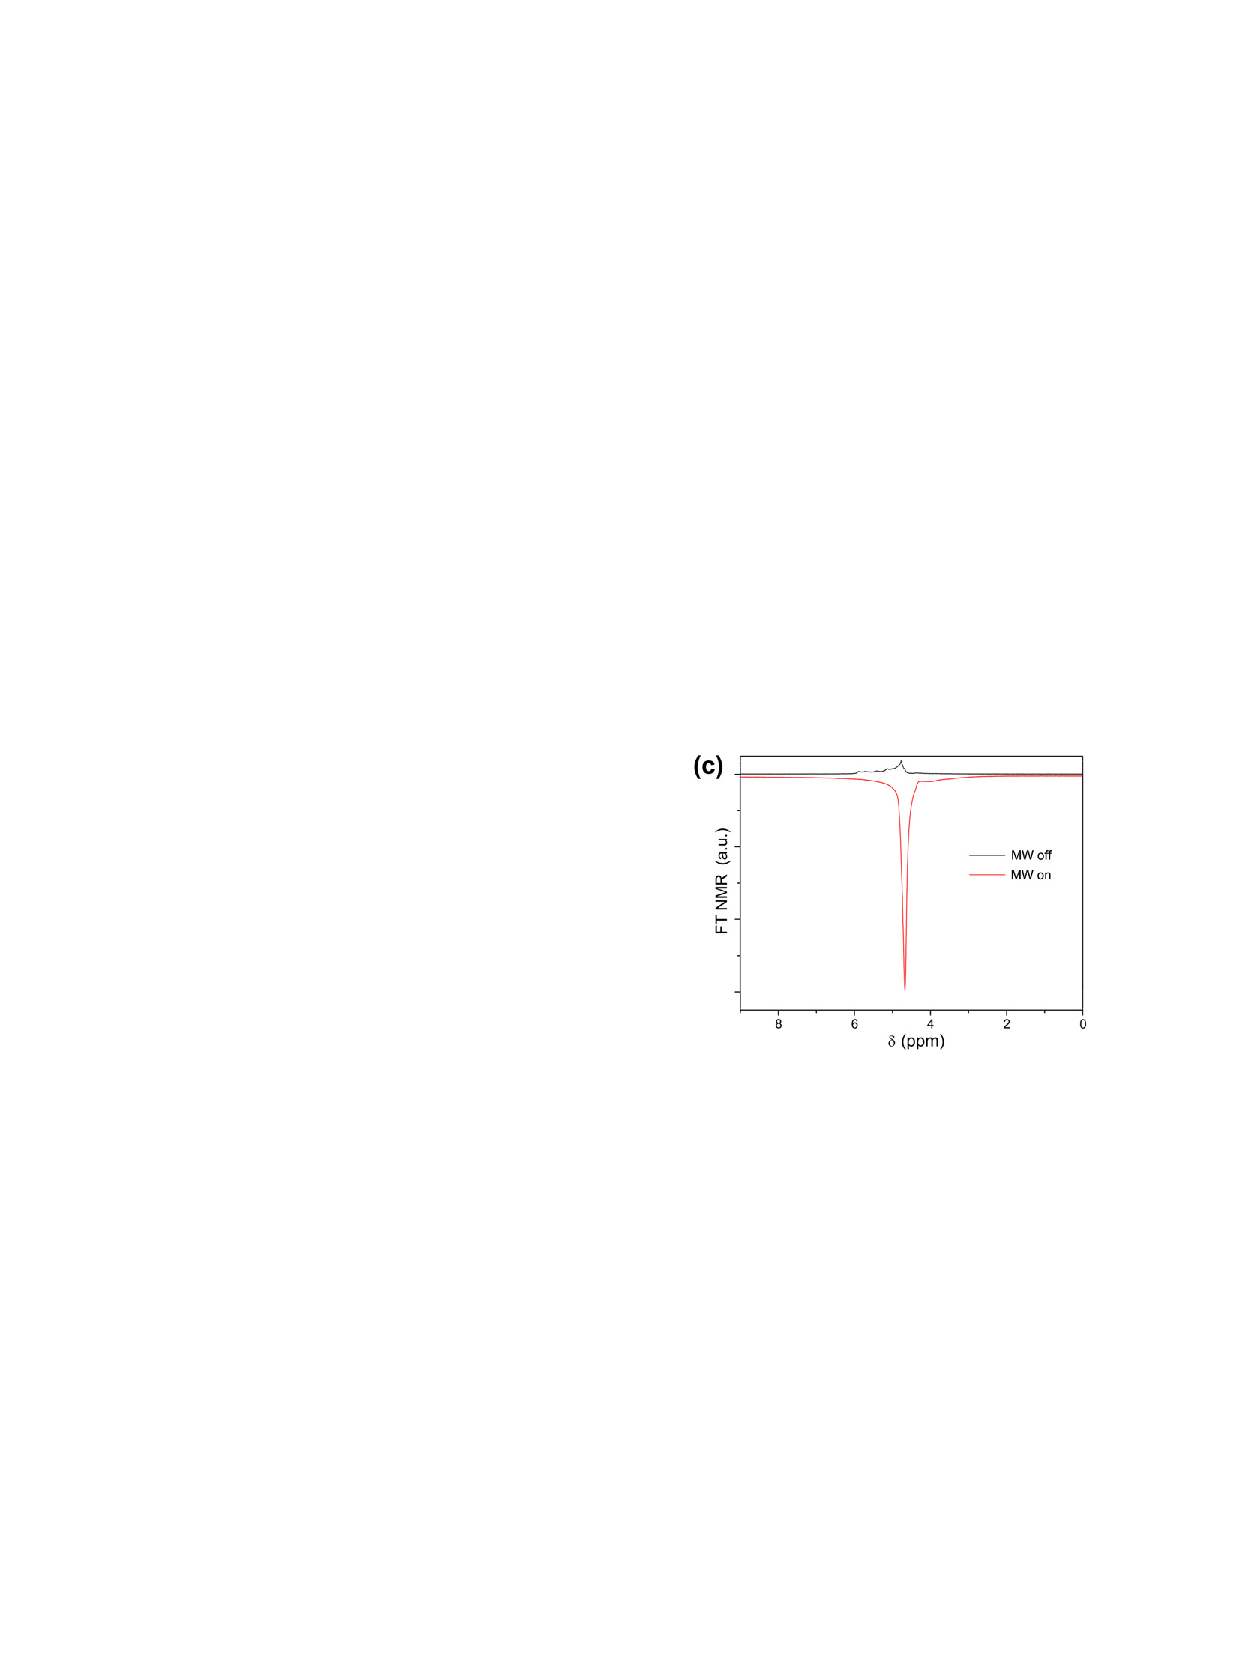
\includegraphics[width=4.cm]{Denysenkov-2012jy-F4c}} ++(-1.8,1) node{};
		\end{tikzpicture}
	\end{center}
	\caption{Liquid-state DNP system based on a Fabry-Perot microwave resonator combined
	with a stripline RF resonator. Adapted with permission from \cite{Denysenkov:2012jy}.}
	\label{fig-Denysenkov-2012jy}
\end{figure}

DNP also works directly in the liquid state. However, the transfer tends to loose
efficiency at high magnetic fields, and the penetration depth of
microwaves at high frequency into most liquids at ambient temperature is
very poor. Nonetheless, there is considerable interest in direct
liquid-state DNP \cite{Loening:2002wg,Lingwood:2009jy,Griffin:2010cu} due
to its conceptual simplicity, and because it could potentially be
applied to systems that cannot tolerate freezing and thawing.
Liquid-state DNP systems are essentially electron-nuclear double
resonance spectrometers, and require irradiation at both the nuclear and
electron Larmor frequencies simultaneously or at least in short
succession. The design of suitable resonators is challenging, since the
low-frequency structure tends to shield the sample from access to the
high-frequency radiation. 

Annino et al
\cite{Annino:2009gd,VillanuevaGaribay:2010cu,vanBentum:2011km} have
designed a dielectric cavity microwave resonator combined with a
waveguide radio frequency resonator based on a pair of straight wires,
operating at a magnetic field of 3.3T. This corresponds to electron and
proton Larmor frequencies of 95 GHz and 150 MHz, respectively. The
microwave power is coupled in through a rectangular waveguide from a
solid state source. At a microwave power of about 70 mW, an enhancement
of the proton signal of -16 was observed in mixture of dioxane and water
containing a nitroxide radical. 

Another design has recently been
presented by Denysenkov et al.
\cite{Denysenkov:2010hy,Denysenkov:2008gf,Denysenkov:2012jy,Prandolini:2009he}
Their system operates at even higher frequencies, with a magnetic field
of 9.2 T (392 MHz NMR / 260 GHz EPR frequencies). They employ a much
more powerful gyrotron microwave source, which is coupled into the DNP
system using a corrugated waveguide. The microwaves emanate from the
waveguide into a Fabry-Perot resonator, the back (mirror) plane of which
is formed by a stripline radio frequency resonator, as shown in \fig{fig-Denysenkov-2012jy}.

The  sample
forms a thin liquid film of 20~$\mu$m thickness and 50~nl volume directly
on the conducting stripline surface. This ensures excellent thermal
contact, and prevents the liquid from heating up too much upon microwave
irradiation. The microwave power employed in Denysenkov's design is
about two orders of magnitude stronger than in the one by Annino et al.
Signal enhancements of up to a factor of 30 have been observed with this
system.
